\chapter{Common Definitions and Conventions}

\section{Coordinate Conventions}
The coordinate system of CMS is centred on the nominal interaction point. The
$x$-axis points towards the centre of the LHC ring, the $y$-axis points vertically
upwards and the $z$-axis points along the direction of the beamline, in the
anti-clockwise direction when the LHC is viewed from above. 
The azimuth angle, $\phi$, is the angle in the $x$-$y$ plane with respect to the
$x$-axis.  The polar angle, $\theta$, is measured from the $z$-axis.

The rapidity of a particle is defined as,
\begin{equation}
    y = \frac{1}{2} \ln \left(\frac{E+p_\text{L}}{E-p_\text{L}}\right),
\label{eq:rapidity}
\end{equation}
where $p_{L}$ is the longitudinal component (the component along the beam axis)
of the momentum of the particle. It represents the boost along the beam axis
required to go from the lab frame to the frame where the particle is produced
perpendicular to the beam axis.
The pseudorapidity is defined as 
\begin{equation}
    \eta = -\ln\left[\tan\left(\frac{\theta}{2}\right)\right], 
\label{eq:pseudorapidity}
\end{equation}
where $\theta$ is the polar angle.  In the massless approximation, this is equal
to the rapidity.
The variable $\Delta R$ is defined as: 
\begin{equation}
  (\Delta R)^{2} = (\Delta \eta)^{2} + (\Delta \phi)^{2} 
  \label{eq:dR}
\end{equation}

In the LHC experiments the initial longitudinal momentum in the event is not
known. Many of the kinematic quantities are considered only in the transverse
($x$-$y$) plane and denoted with a `T' subscript, for example the transverse
missing energy, \ETm, and the transverse momentum, \pT.

\section{List of Acronyms}
\begin{center}
\begin{longtable}{ll}
ALICE\dotfill & A Large Ion Collider Experiment\\
APD\dotfill & Avalanche Photodiode\\
AS\dotfill & Anti-Selection\\
ATLAS\dotfill & A Toroidal LHC ApparatuS\\
CERN\dotfill & European Organisation for Nuclear Research.\\
CMS\dotfill & Compact Muon Solenoid\\
CPU\dotfill & Central Processing Unit\\
CSC\dotfill & Cathode Strip Chamber\\
CTEQ\dotfill & The Coordinated Theoretical-Experimental Project on QCD\cite{lai2010vv}\\
DAQ\dotfill & Data Acquisition\\
DT\dotfill & Drift Tube\\
DY\dotfill & Drell-Yan\\
ECAL\dotfill & Electromagnetic Calorimeter\\
\ETm\dotfill & Missing Transverse Energy\\
EWSB\dotfill & Electroweak Symmetry Breaking\\
FSR\dotfill & Final State Radiation.\\
GSF\dotfill & Gaussian Sum Filter\\
HCAL\dotfill & Hadronic Calorimeter\\
HEP\dotfill & High Energy Physics\\
HERAPDF\dotfill & Hadron Elektron Ring Anlage PDF\cite{aaron2010combined} \\
HF\dotfill & Hadronic Calorimeter (Forward)\\
HLT\dotfill & High Level Trigger\\
KF\dotfill & Kalman Filter\\
L1\dotfill & Level 1 Trigger\\
LEP\dotfill & Large Electron-Positron Collider\\
LHAPDF\dotfill & Les Houches Accord PDF Interface\cite{whalley2005houches}\\
LHCb\dotfill & Large Hadron Collider Beauty.\\
LHC\dotfill & Large Hadron Collider\\
LINAC2\dotfill & Linear Accelerator 2\\
MC\dotfill & Monte Carlo\\
MCFM\dotfill & Monte Carlo for FeMtobarn processes\cite{campbellmcfm}\\
MET\dotfill & Missing Transverse Energy\\
MSTW\dotfill & Martin-Stirling-Thorne-Watt Parton Distribution Functions\cite{martin2009parton}\\
MVA\dotfill & Multivariate Analysis\\
NNPDF\dotfill & Neural Network Parton Distribution Functions\cite{Lionetti:2011pw}\\
NP\dotfill & New Physics\\
PDF\dotfill & Parton Distribution Function\\
PF\dotfill & Particle Flow\\
PFMET\dotfill & Particle Flow Missing Transverse Energy\\
PSB\dotfill & Proton Synchrotron Booster\\
PS\dotfill & Proton Synchrotron\\
PU\dotfill & Pile Up\\
PV\dotfill & Primary Vertex\\
QCD\dotfill & Quantum ChromoDynamics\\
QED\dotfill & Quantum ElectroDynamics\\
RPC\dotfill & Resistive Plate Chamber\\
SM\dotfill & Standard Model\\
SPS\dotfill & Super Proton Synchrotron\\
SUSY\dotfill & Supersymmetry\\
TEC\dotfill & Tracker End Cap\\
TIB\dotfill & Tracker Inner Barrel\\
TID\dotfill & Tracker Inner Disk\\
TOB\dotfill & Tracker Outer Barrel.\\
TP\dotfill & Tag and Probe\\
VEV\dotfill & Vacuum Expectation Value\\
VPT\dotfill & Vacuum Phototriode\\
\end{longtable}
\end{center}

\chapter{Fits to the \ETm Distributions}
\section{\unit{36}{\invpb}}

The following plots show the results of the fits to the \ETm for each
pseudorapidity/charge bin with \unit{36}{\invpb} of data. The $x$-axis is the
particle flow \ETm (GeV) and the $y$-axis is the number of events. The results
are for the $\Pt > \unit{25}{\GeV}$ cut.

\begin{figure}
\begin{center}
% bottom right top left
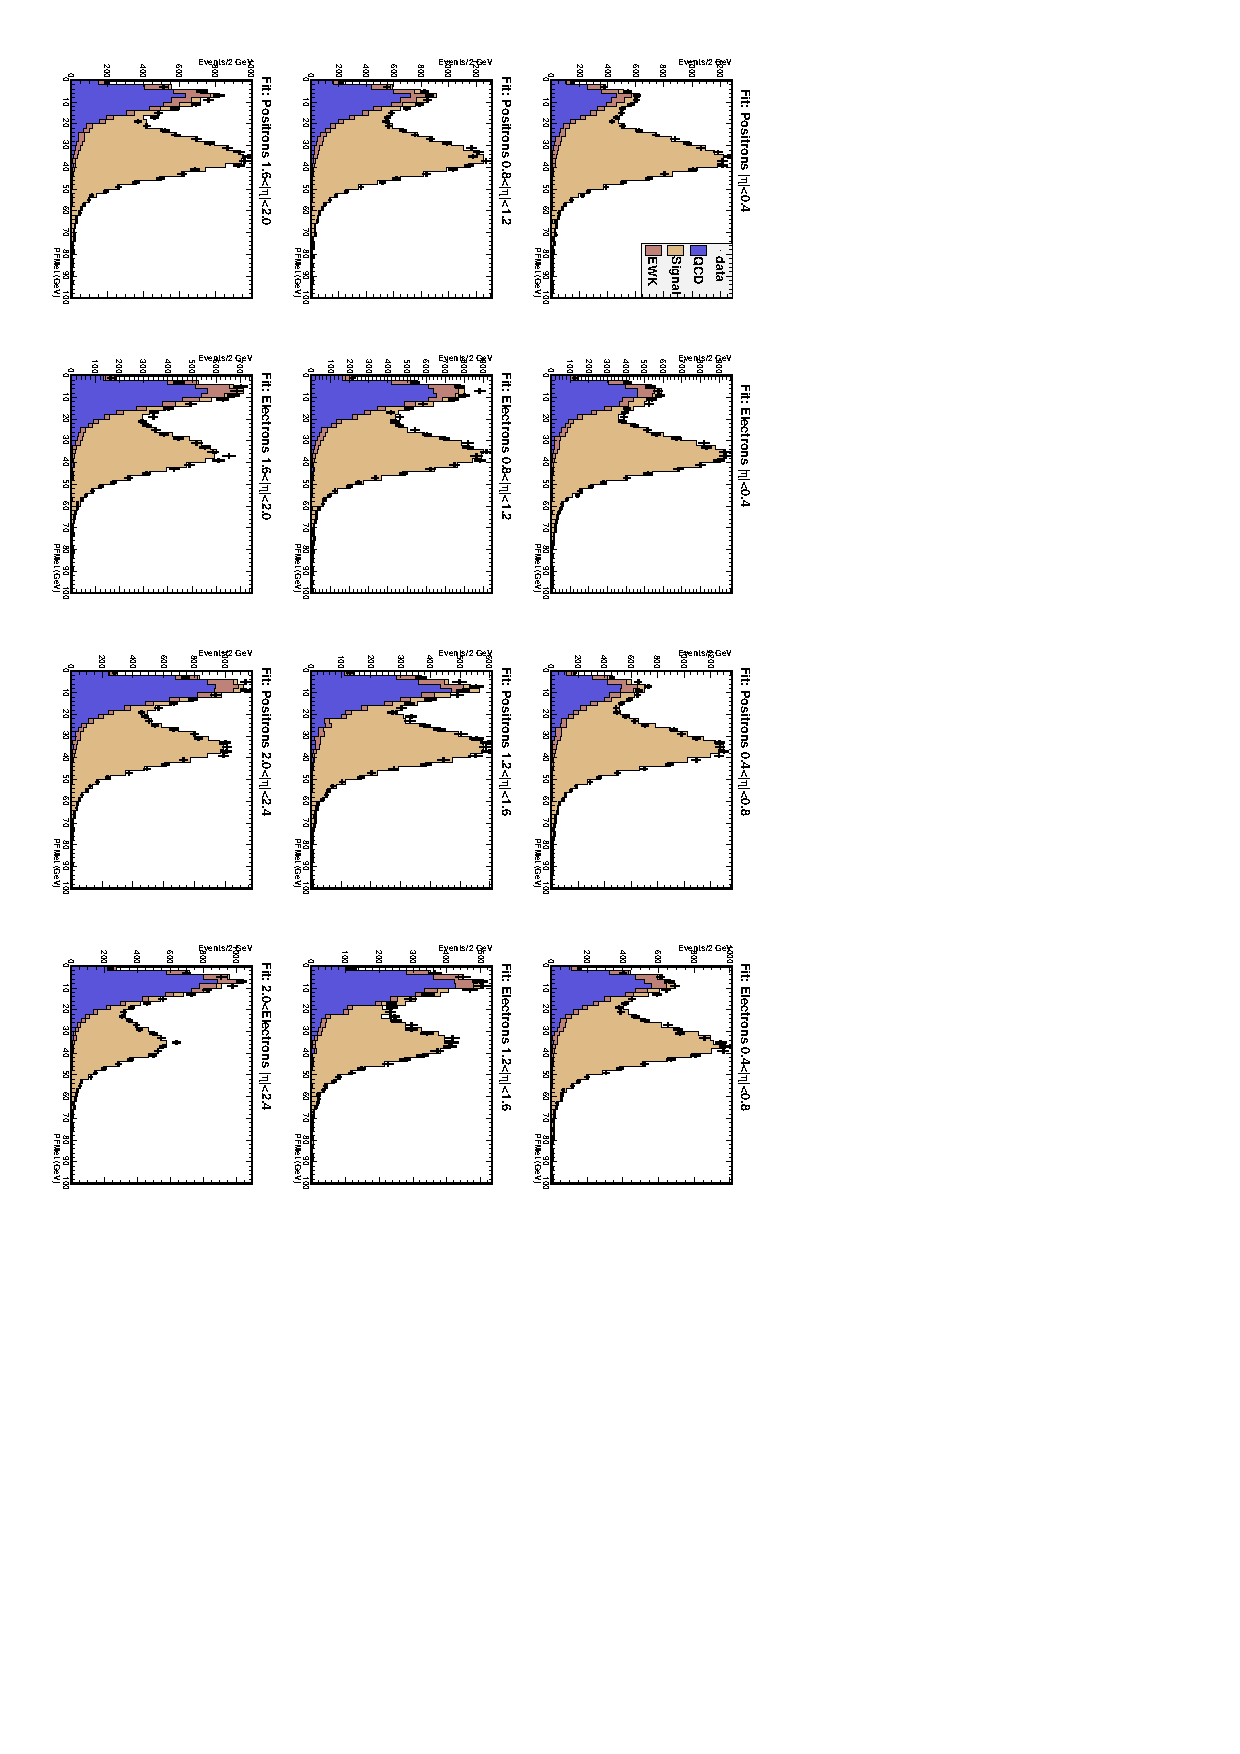
\includegraphics[trim = 80mm 100mm 0mm 0mm, clip, angle=90, width=0.95\textwidth]{Dec22_data}
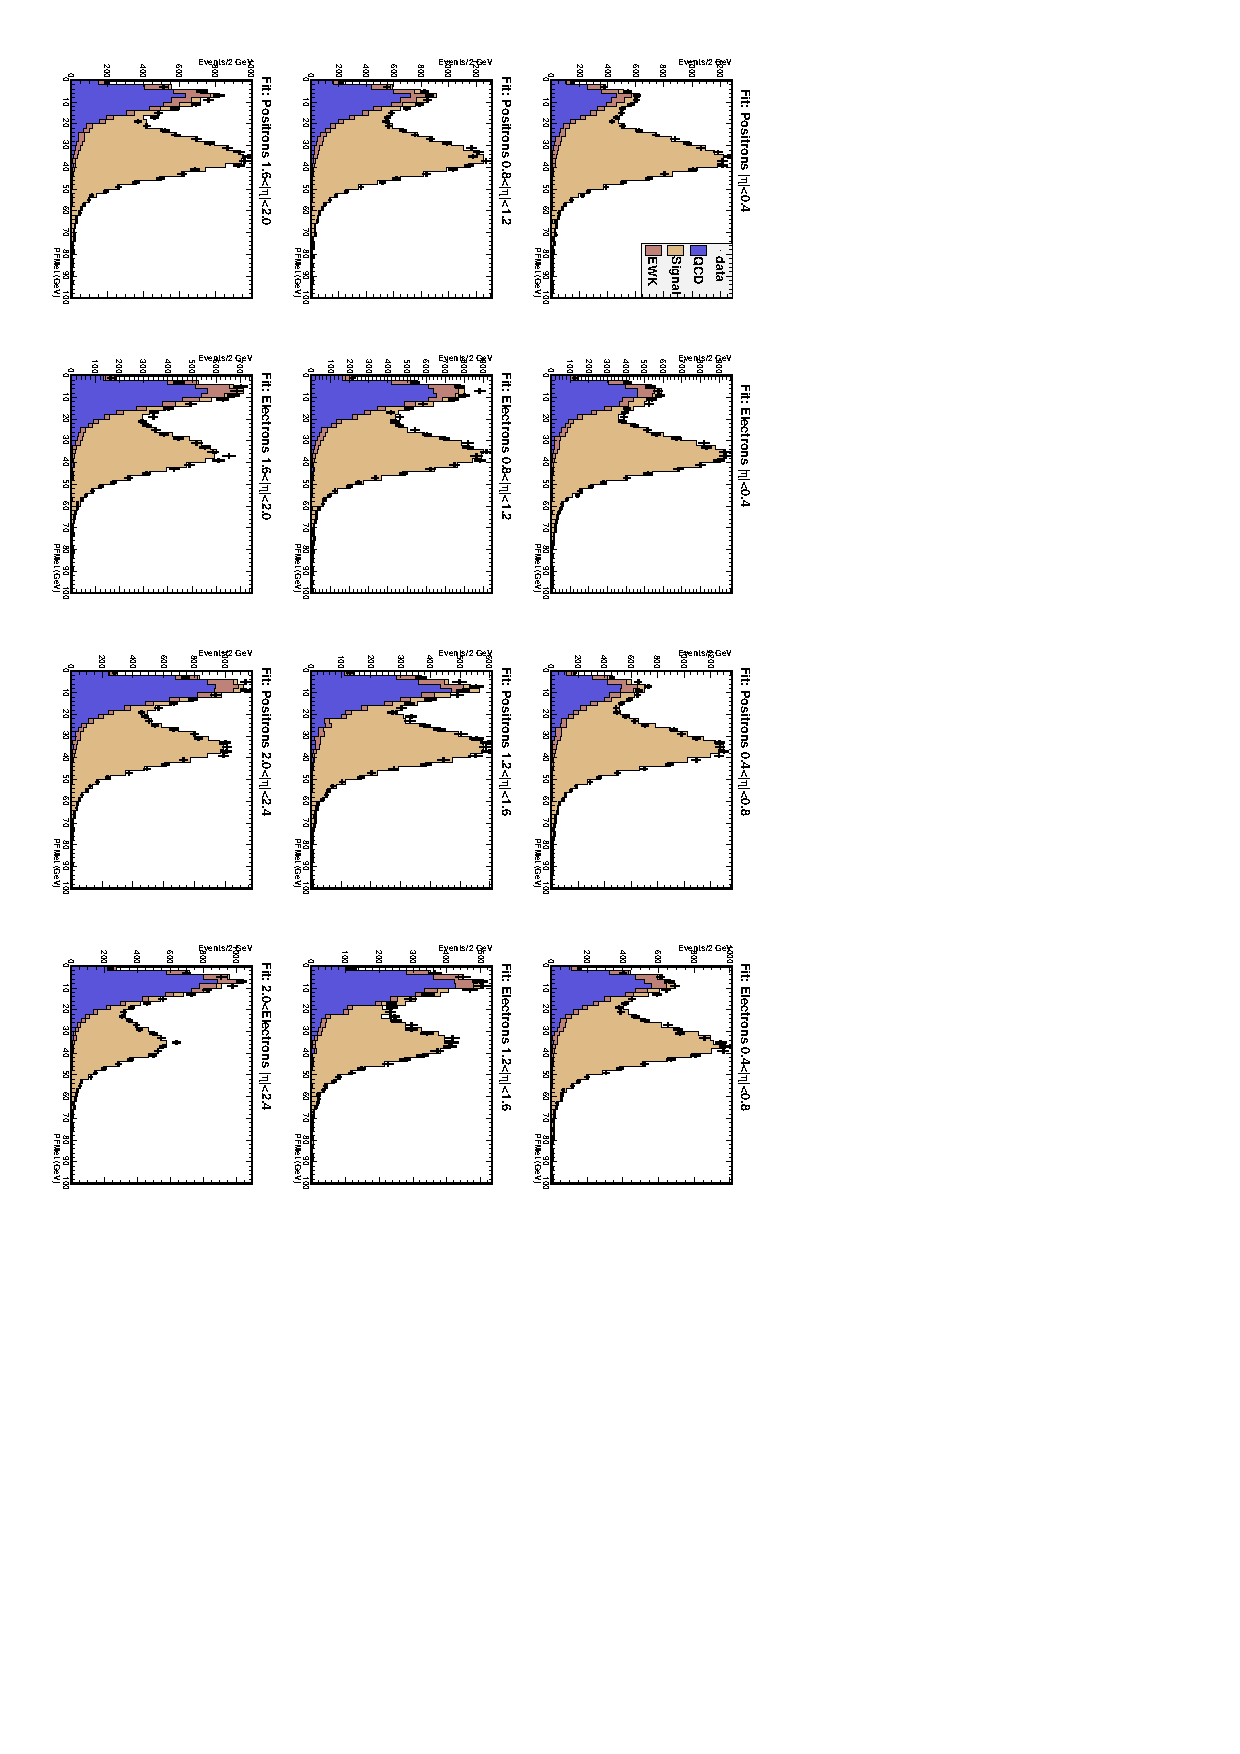
\includegraphics[trim = 80mm 0mm 0mm 100mm, clip, angle=90, width=0.95\textwidth]{Dec22_data}
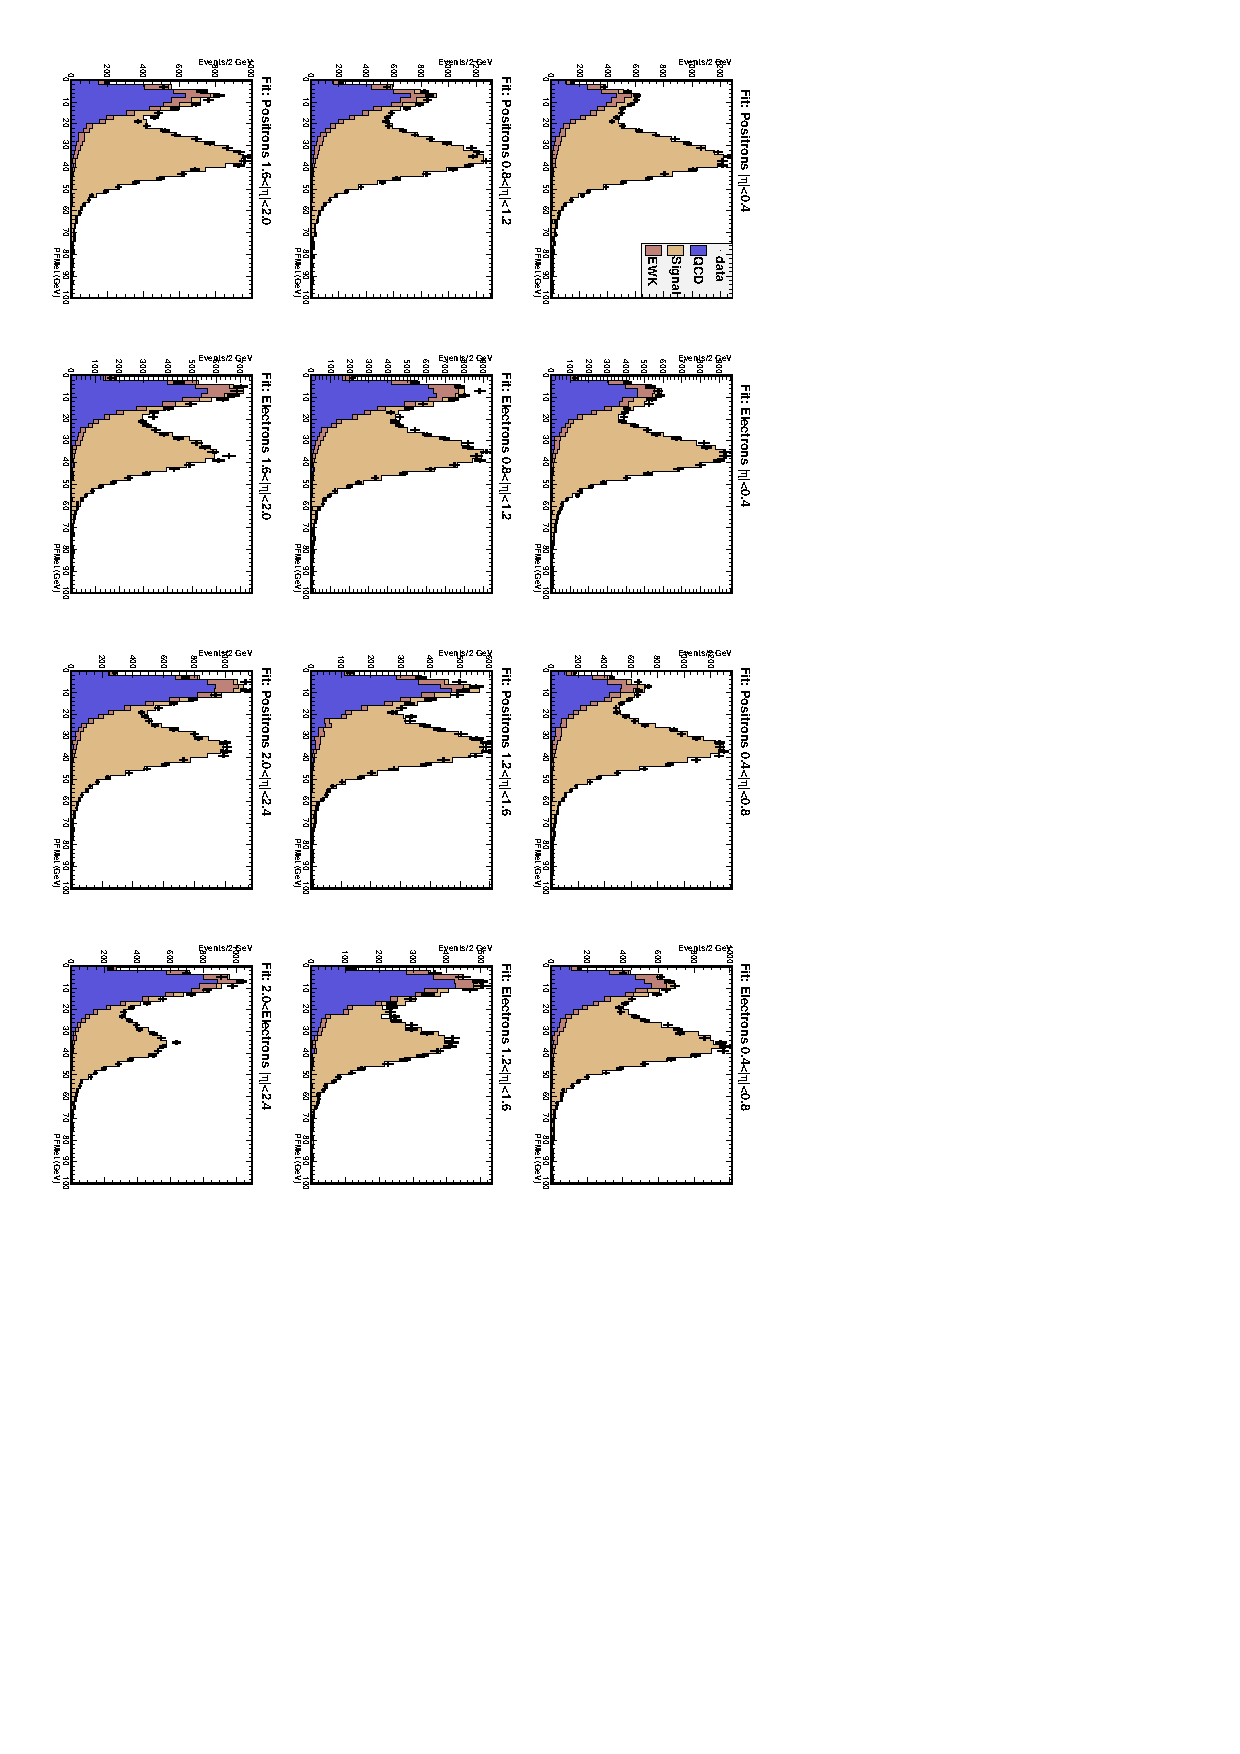
\includegraphics[trim = 40mm 100mm 40mm 0mm, clip, angle=90, width=0.95\textwidth]{Dec22_data}
\caption[The fit to \ETm for each pseudorapidity/charge bin.] {\label{fig:fit1}
The fit to \ETm\ for each pseudorapidity/charge bin.  The $x$-axis is the
particle flow \ETm (GeV) and the $y$-axis is the number of events
($2\GeV^{-1}$).}
\end{center}
\end{figure}

\begin{figure}
\begin{center}
% bottom right top left
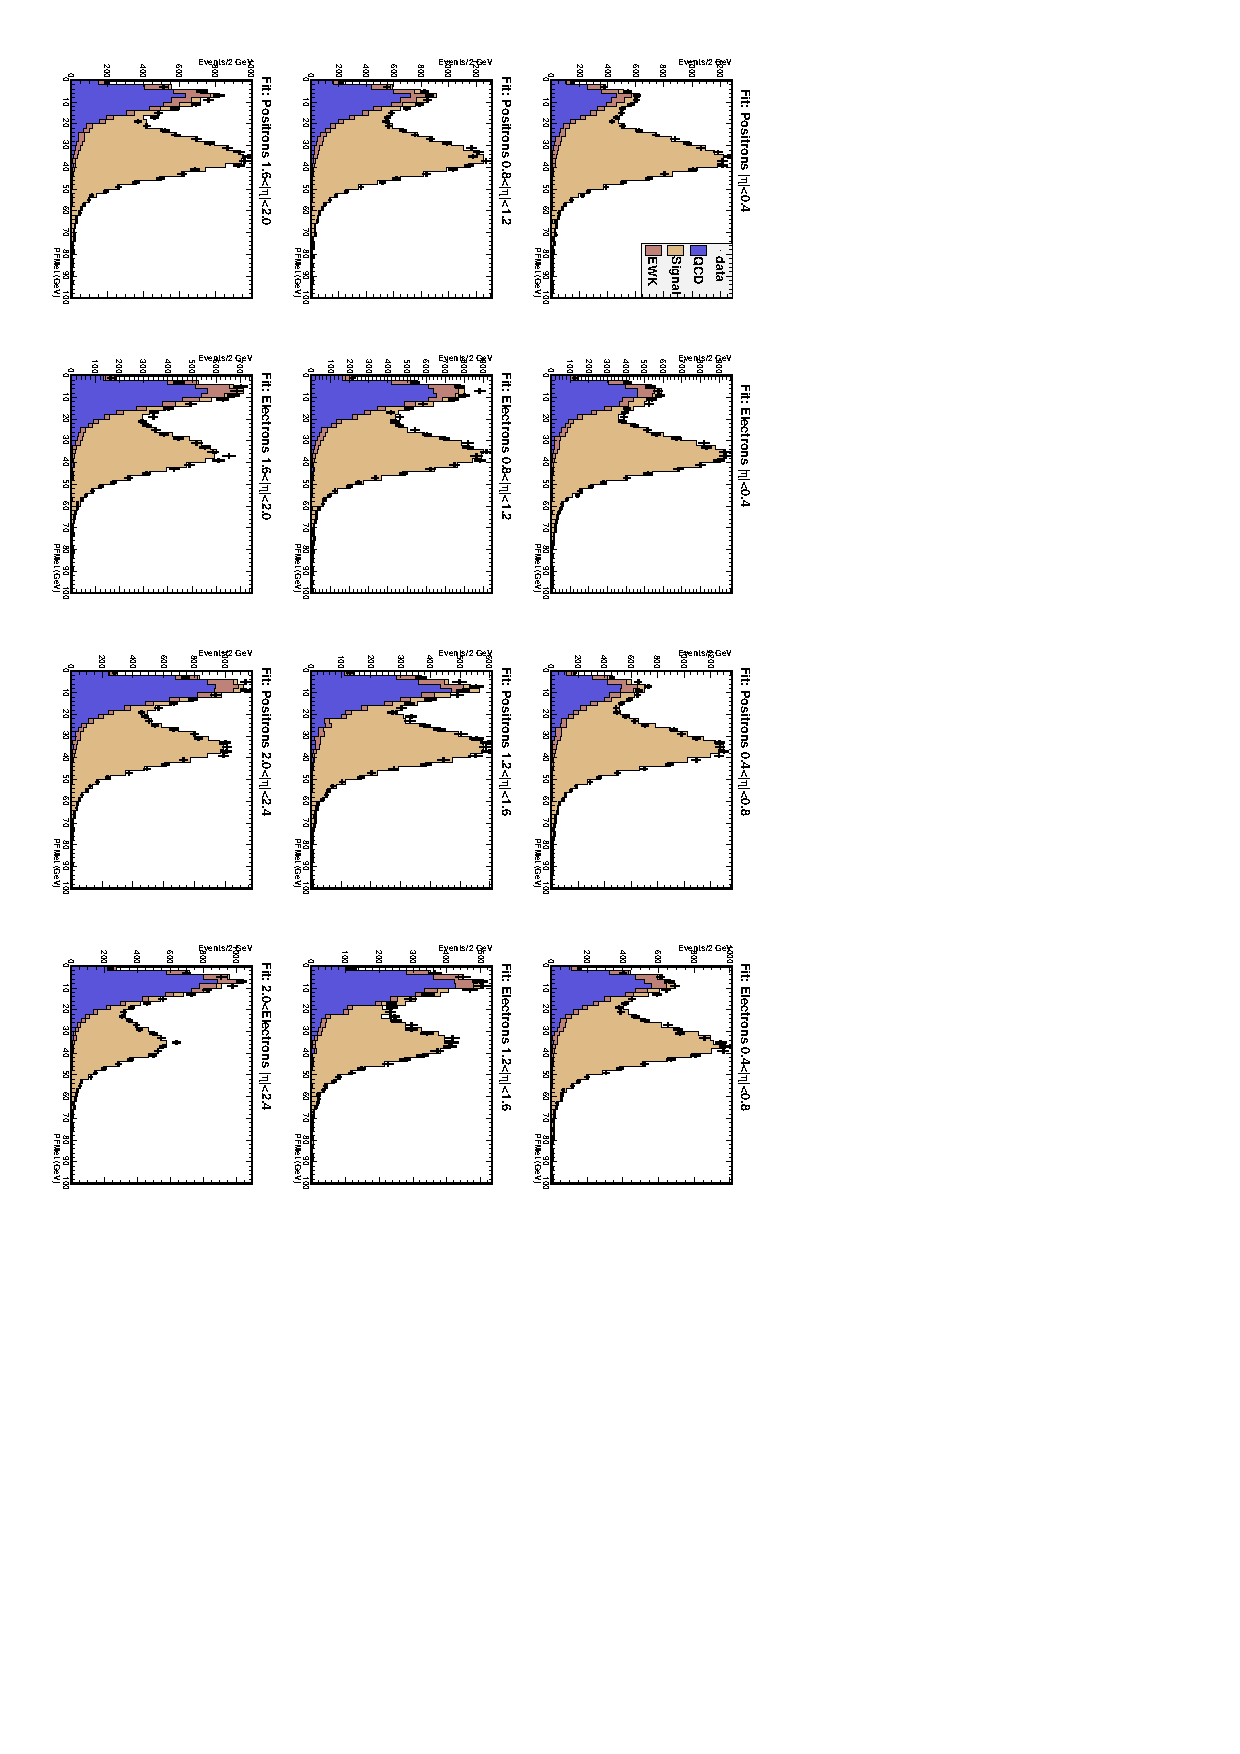
\includegraphics[trim = 40mm 0mm 40mm 100mm, clip, angle=90, width=0.95\textwidth]{Dec22_data}
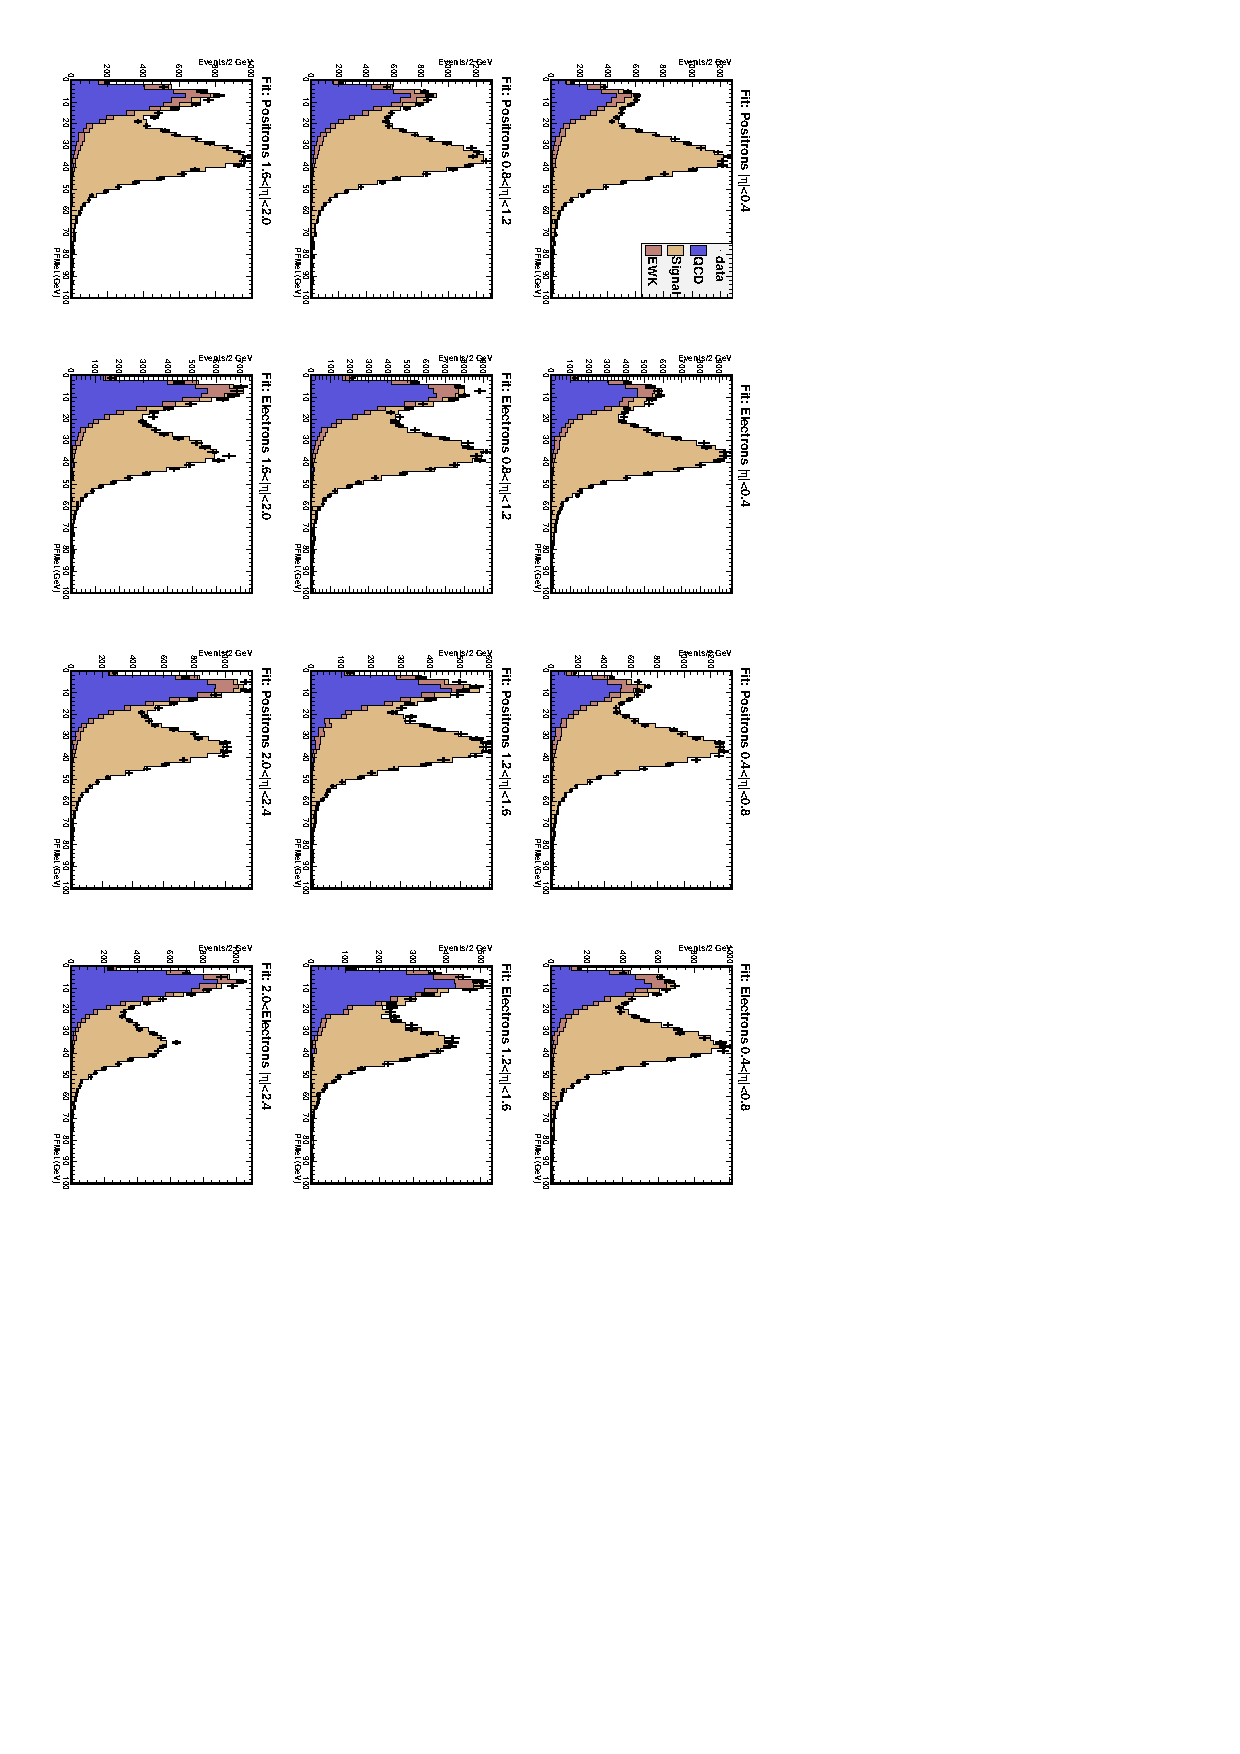
\includegraphics[trim = 0mm 100mm 80mm 0mm, clip, angle=90, width=0.95\textwidth]{Dec22_data}
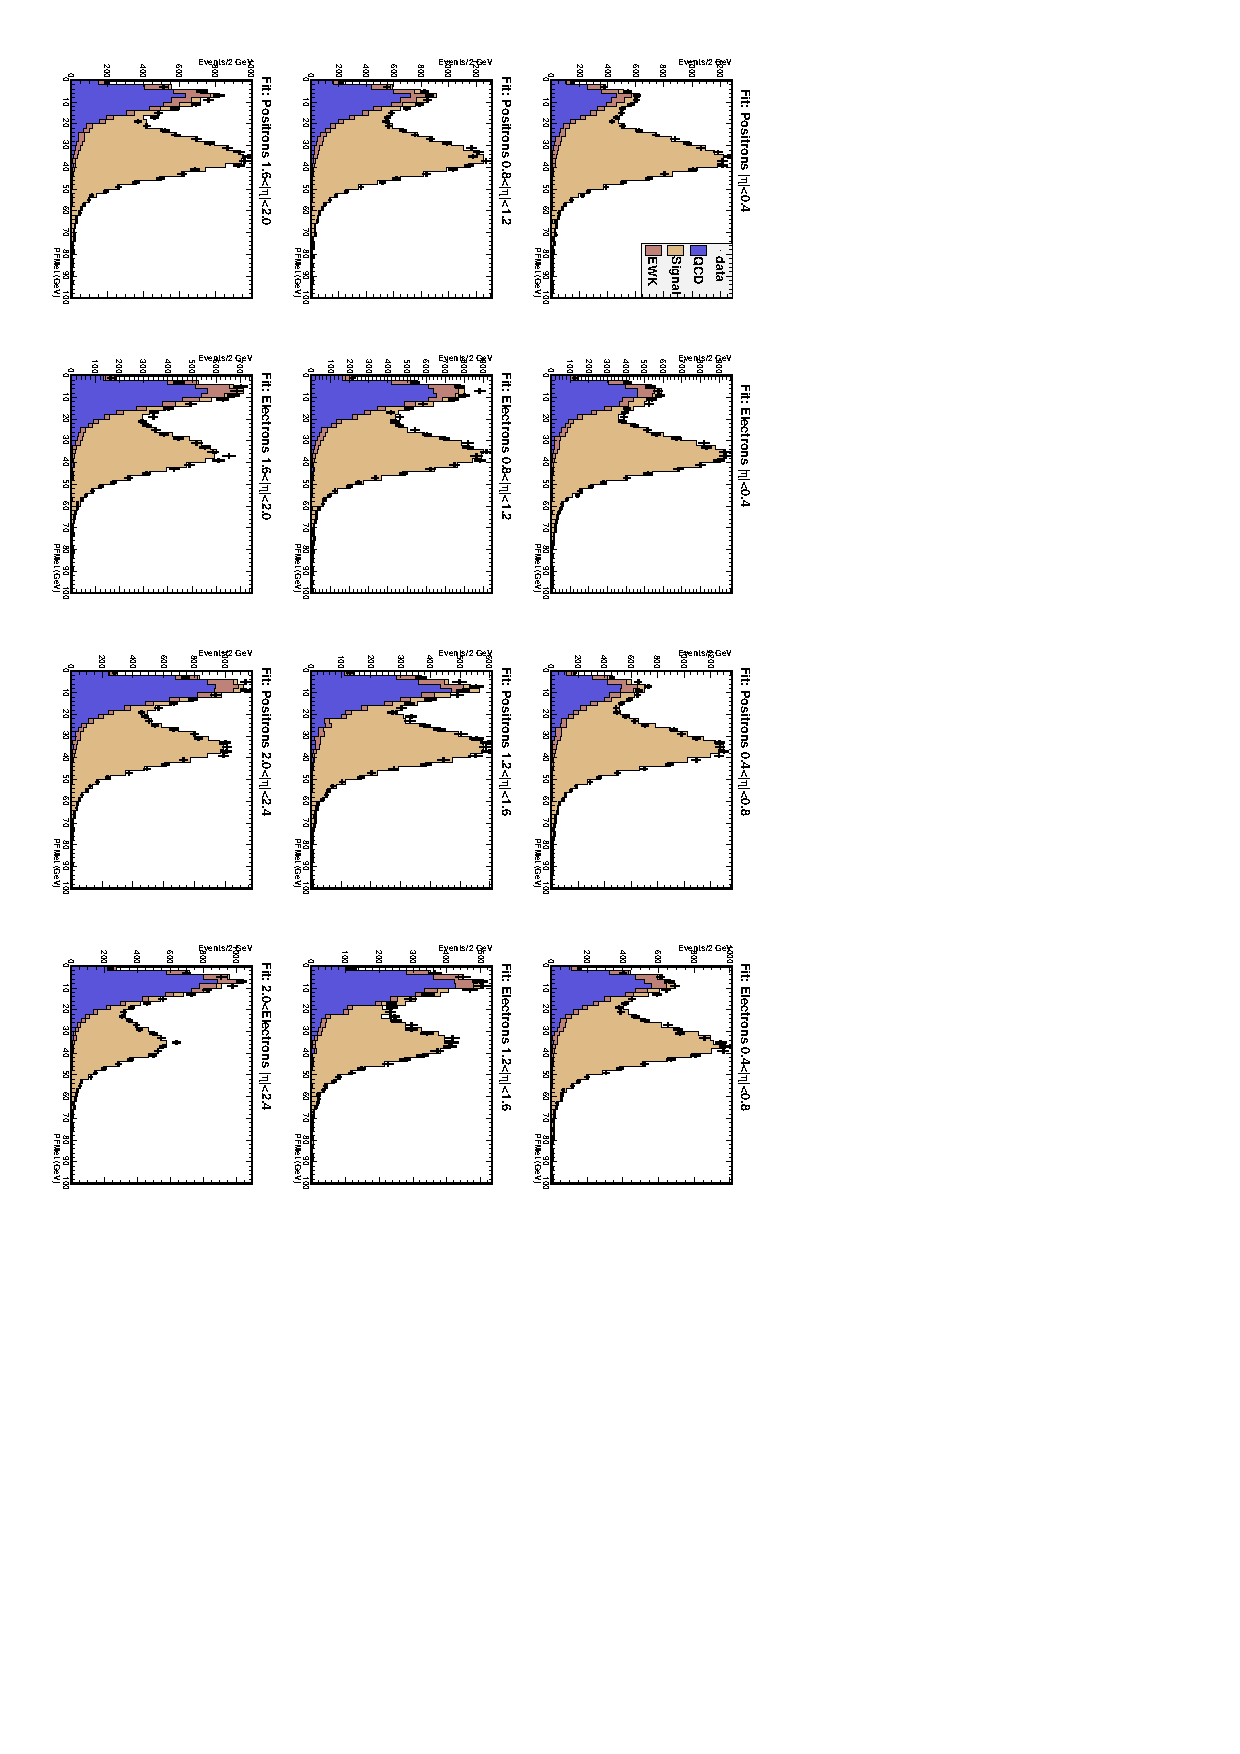
\includegraphics[trim = 0mm 0mm 80mm 100mm, clip, angle=90, width=0.95\textwidth]{Dec22_data}
\caption[The fit to \ETm\ for each pseudorapidity/charge bin.]
{\label{fig:fit2} The fit to \ETm\ for each pseudorapidity/charge
bin.  The $x$-axis is the particle flow \ETm (GeV) and the $y$-axis is the
number of events ($2\GeV^{-1}$).}
\end{center}
\end{figure}

%\begin{figure}
%\begin{center}
% bottom right top left
%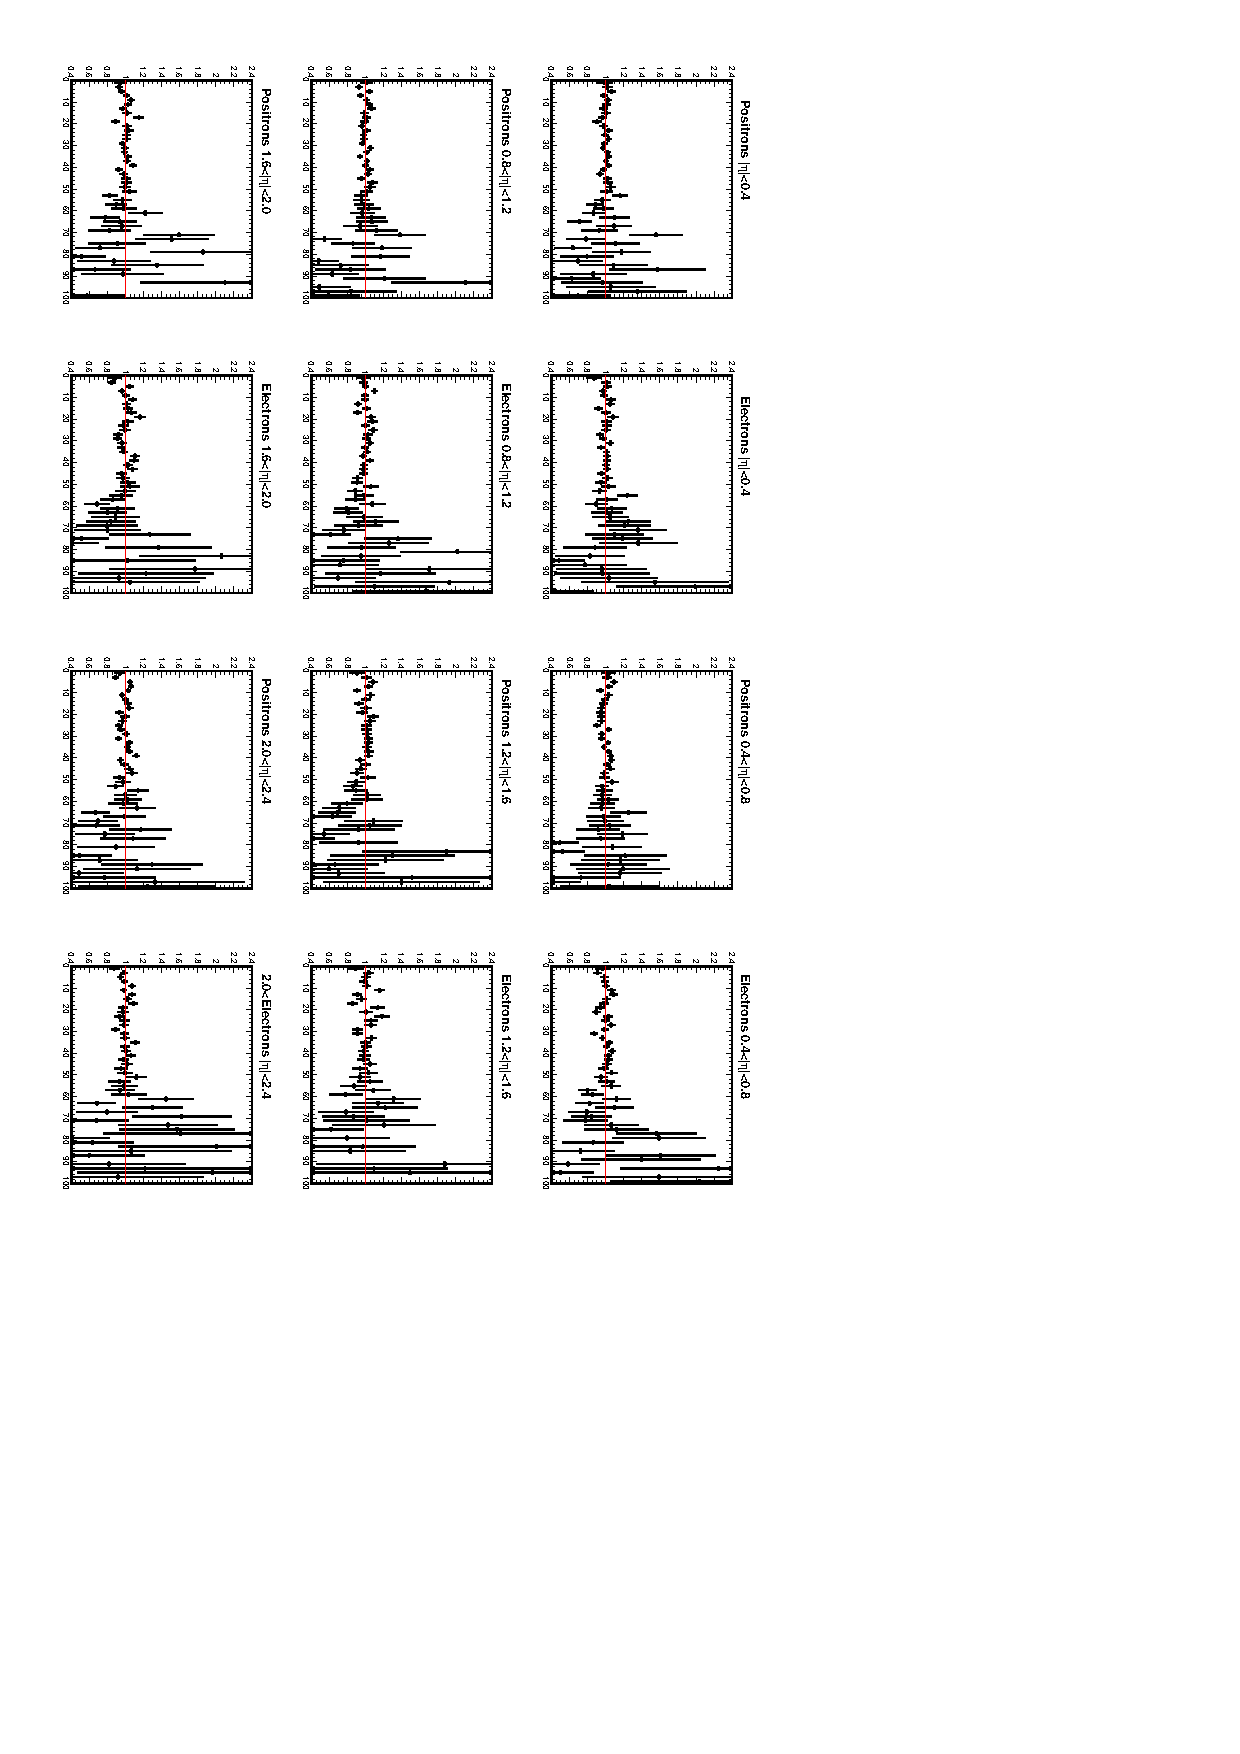
\includegraphics[trim = 80mm 100mm 0mm 0mm, clip, angle=90, width=0.95\textwidth]{Dec22_fitratio}
%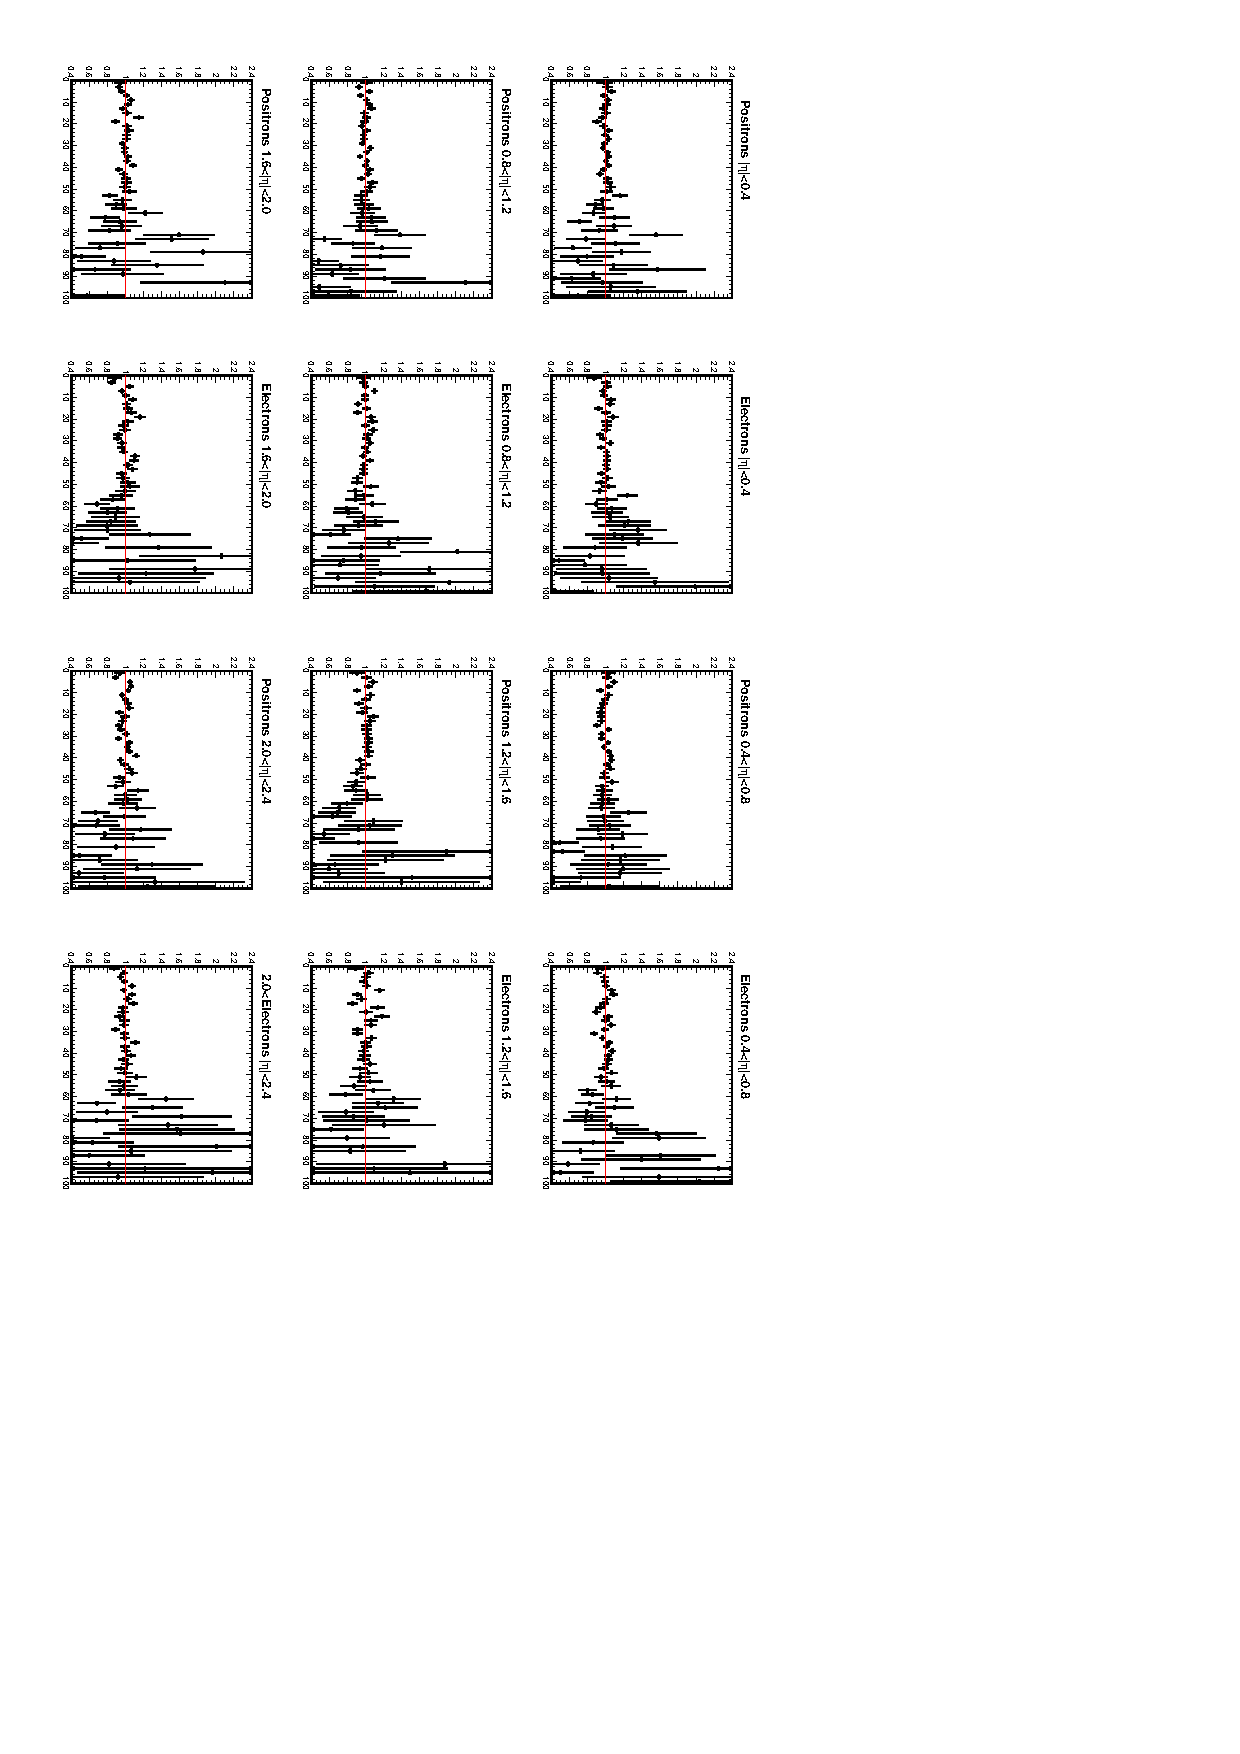
\includegraphics[trim = 80mm 0mm 0mm 100mm, clip, angle=90, width=0.95\textwidth]{Dec22_fitratio}
%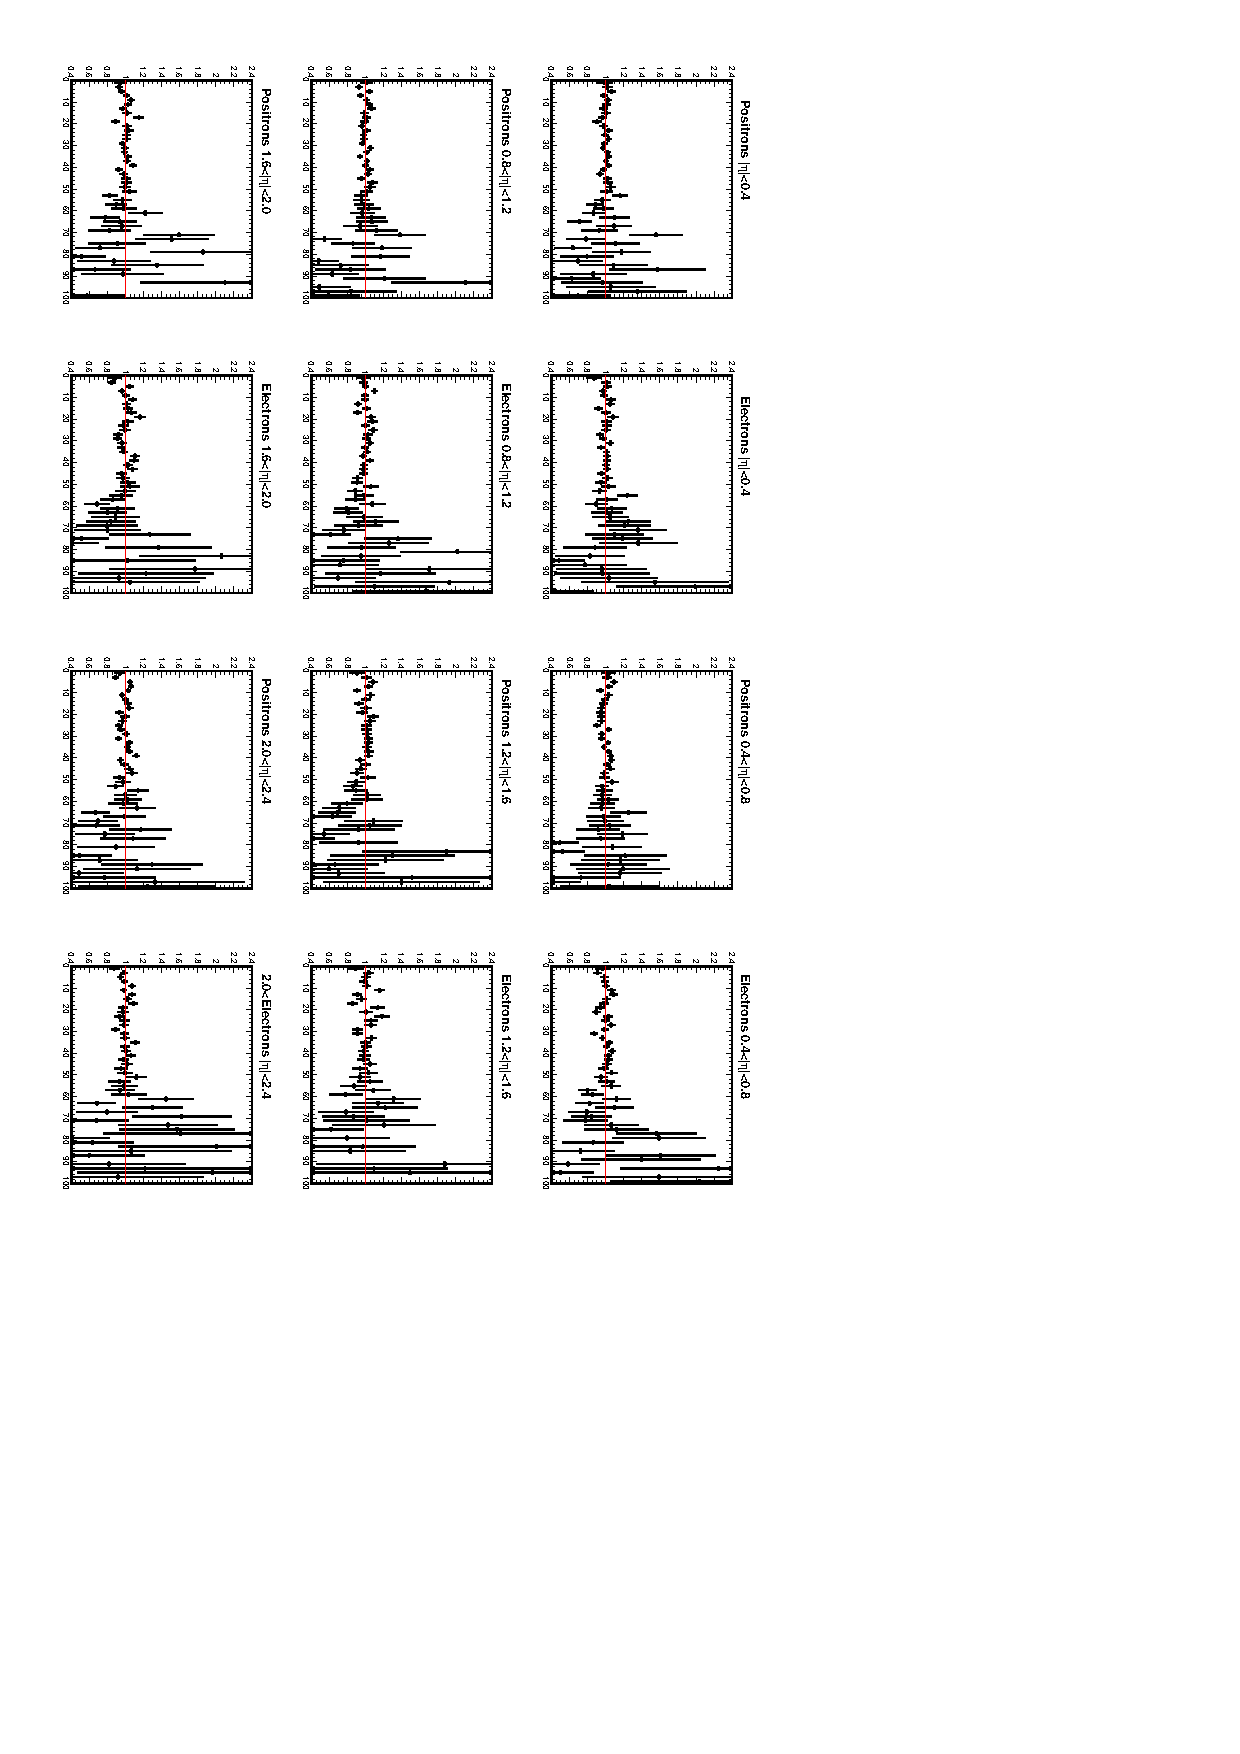
\includegraphics[trim = 40mm 100mm 40mm 0mm, clip, angle=90, width=0.95\textwidth]{Dec22_fitratio}
%\caption{\label{fig:fit1ratio}Ratio between fit and data for each pseudorapidity/charge bin.
%The $x$-axis is the particle flow \ETm (GeV).}
%\end{center}
%\end{figure}

%\begin{figure}
%\begin{center}
%% bottom right top left
%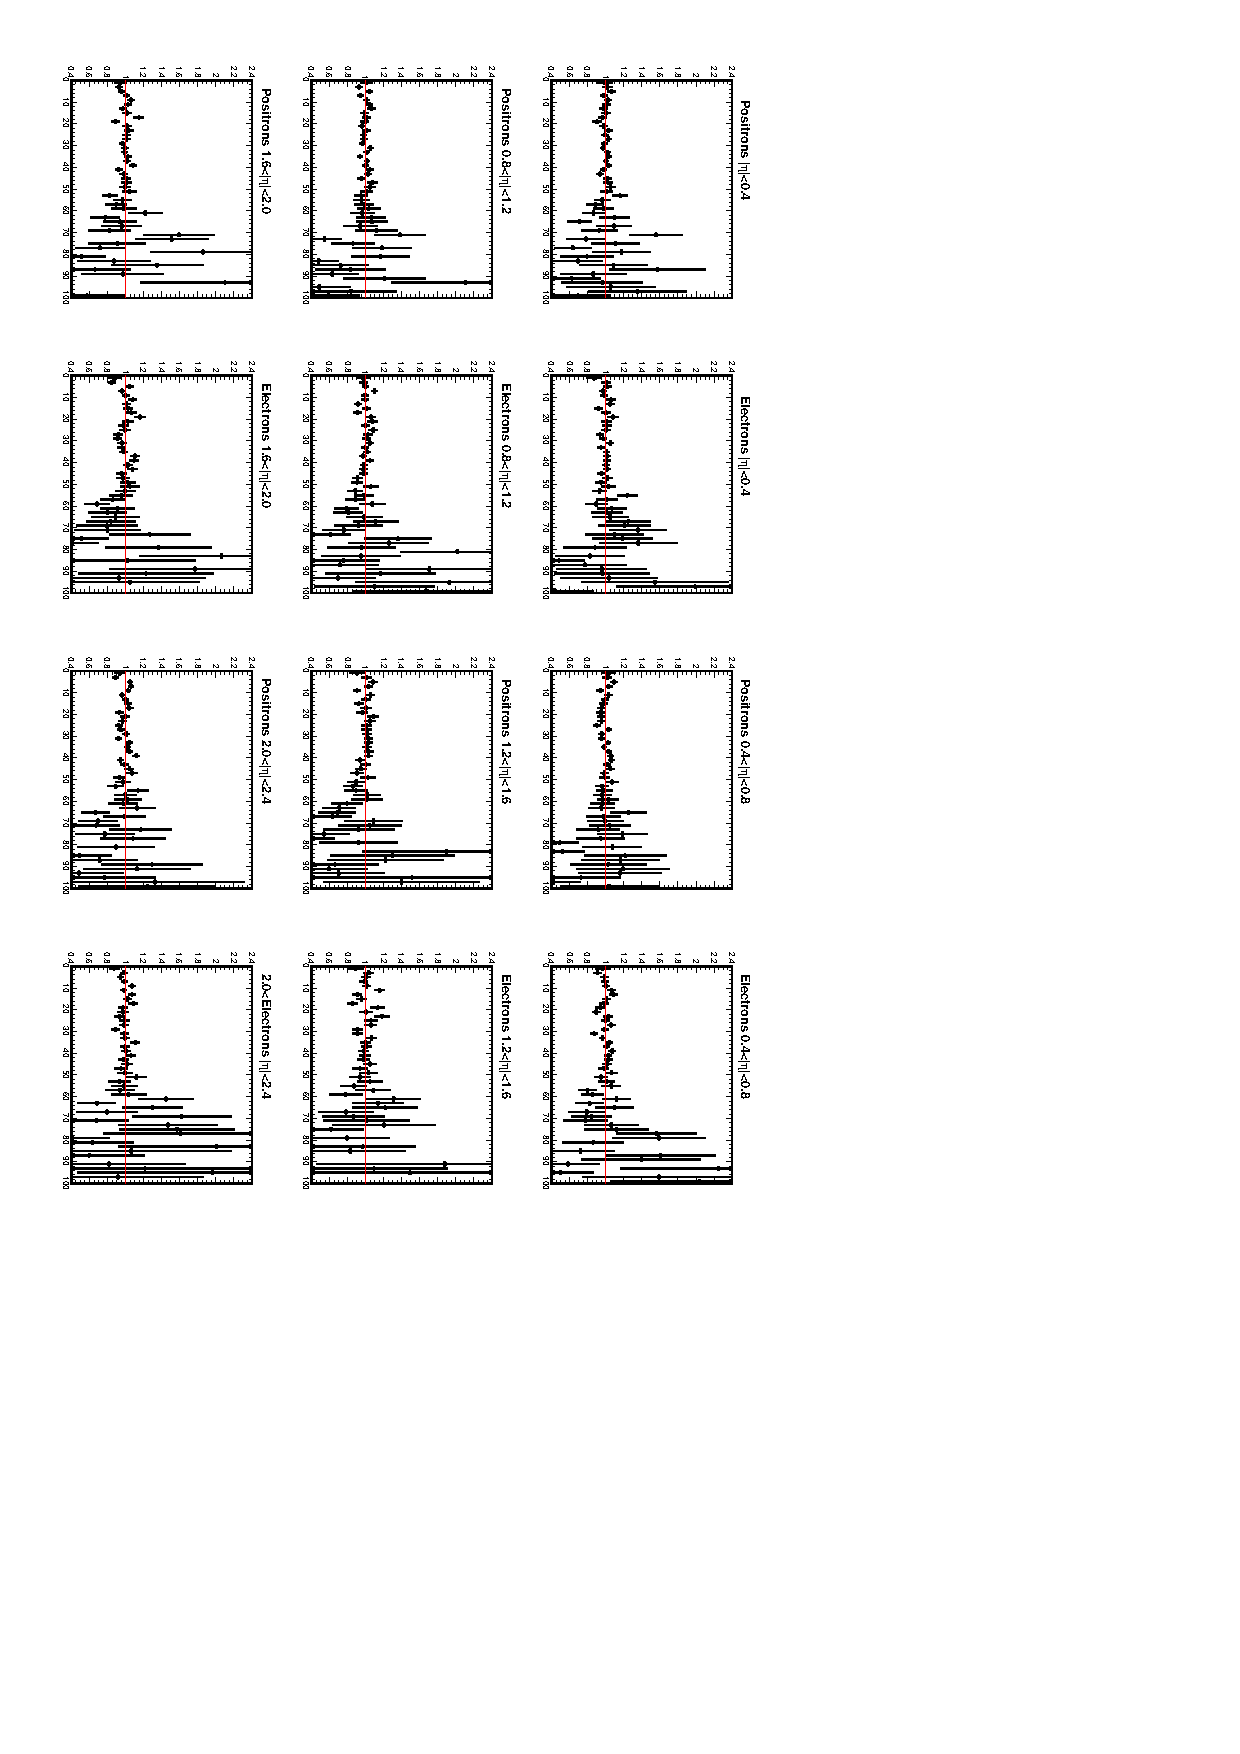
\includegraphics[trim = 40mm 0mm 40mm 100mm, clip, angle=90, width=0.95\textwidth]{Dec22_fitratio}
%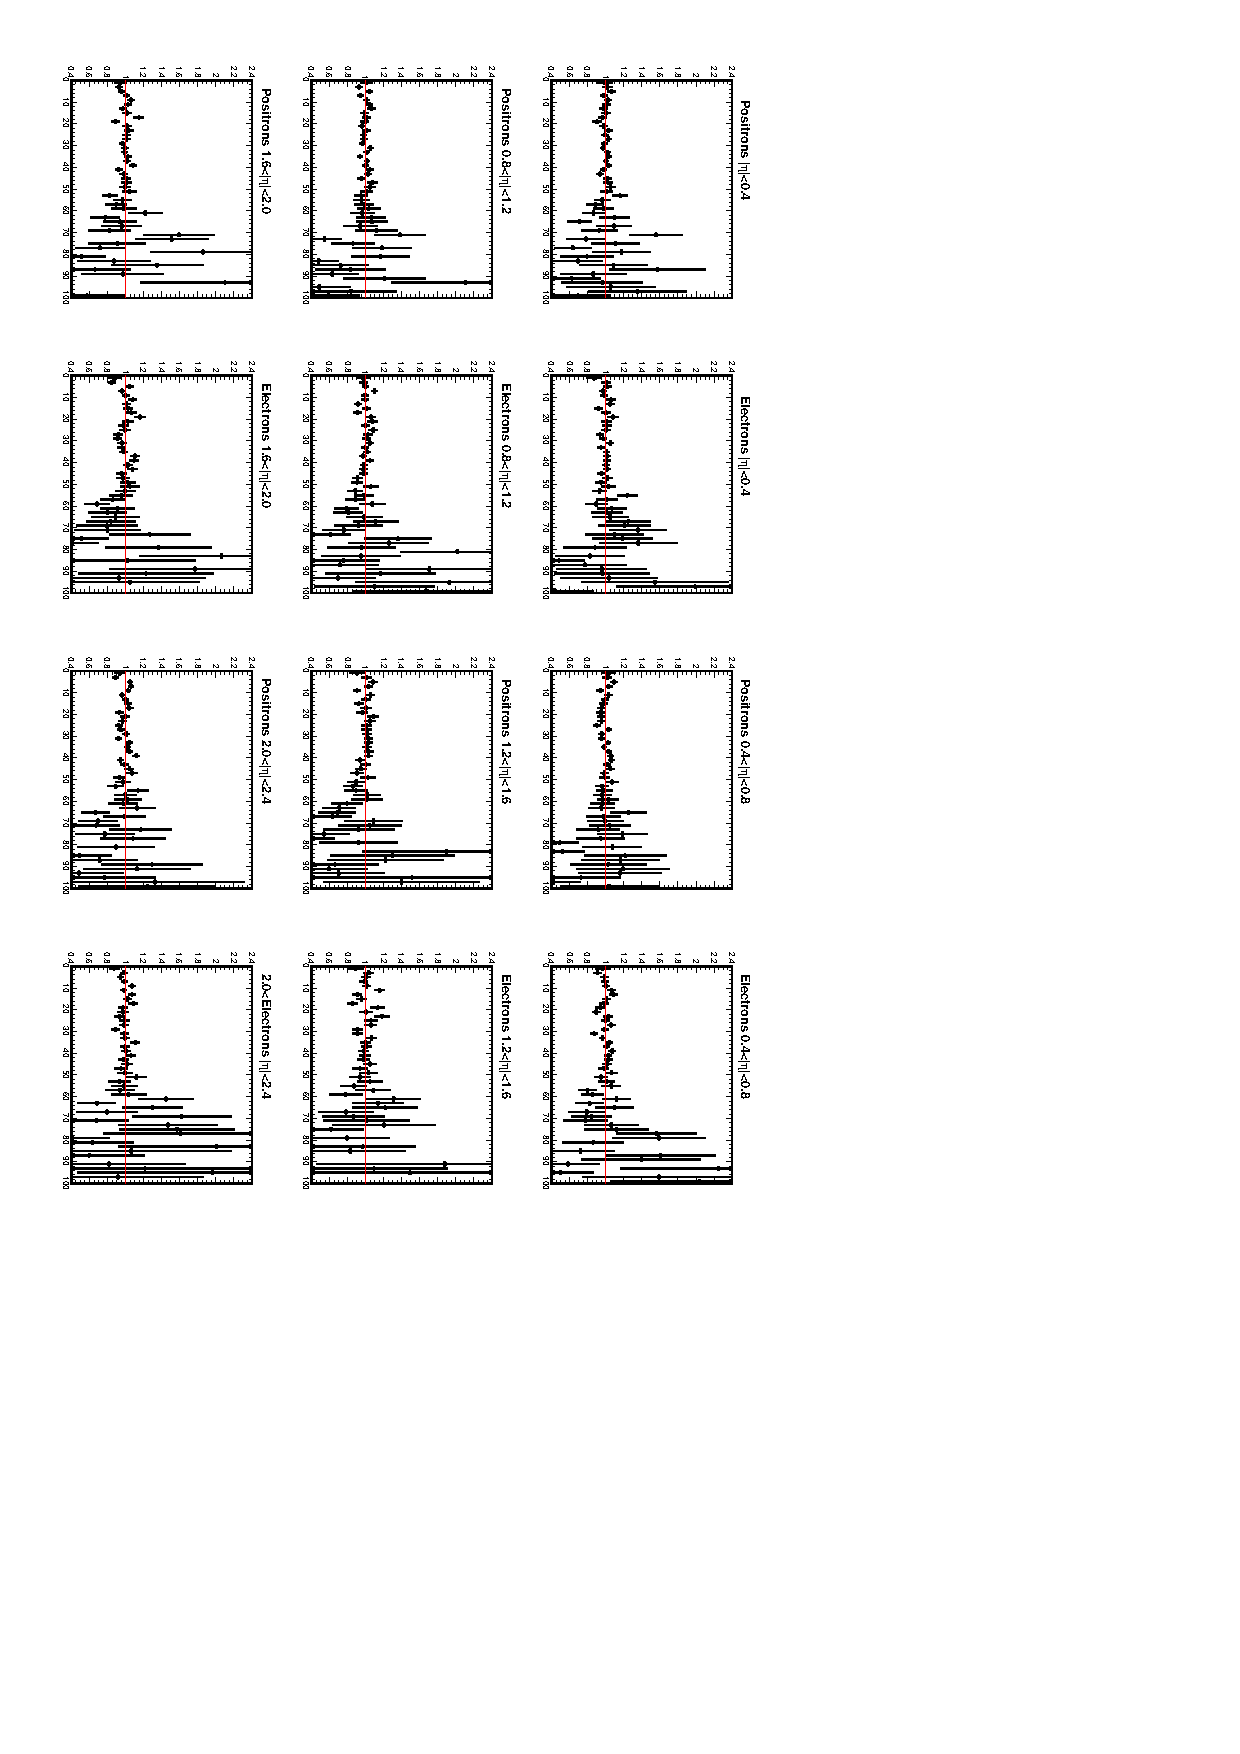
\includegraphics[trim = 0mm 100mm 80mm 0mm, clip, angle=90, width=0.95\textwidth]{Dec22_fitratio}
%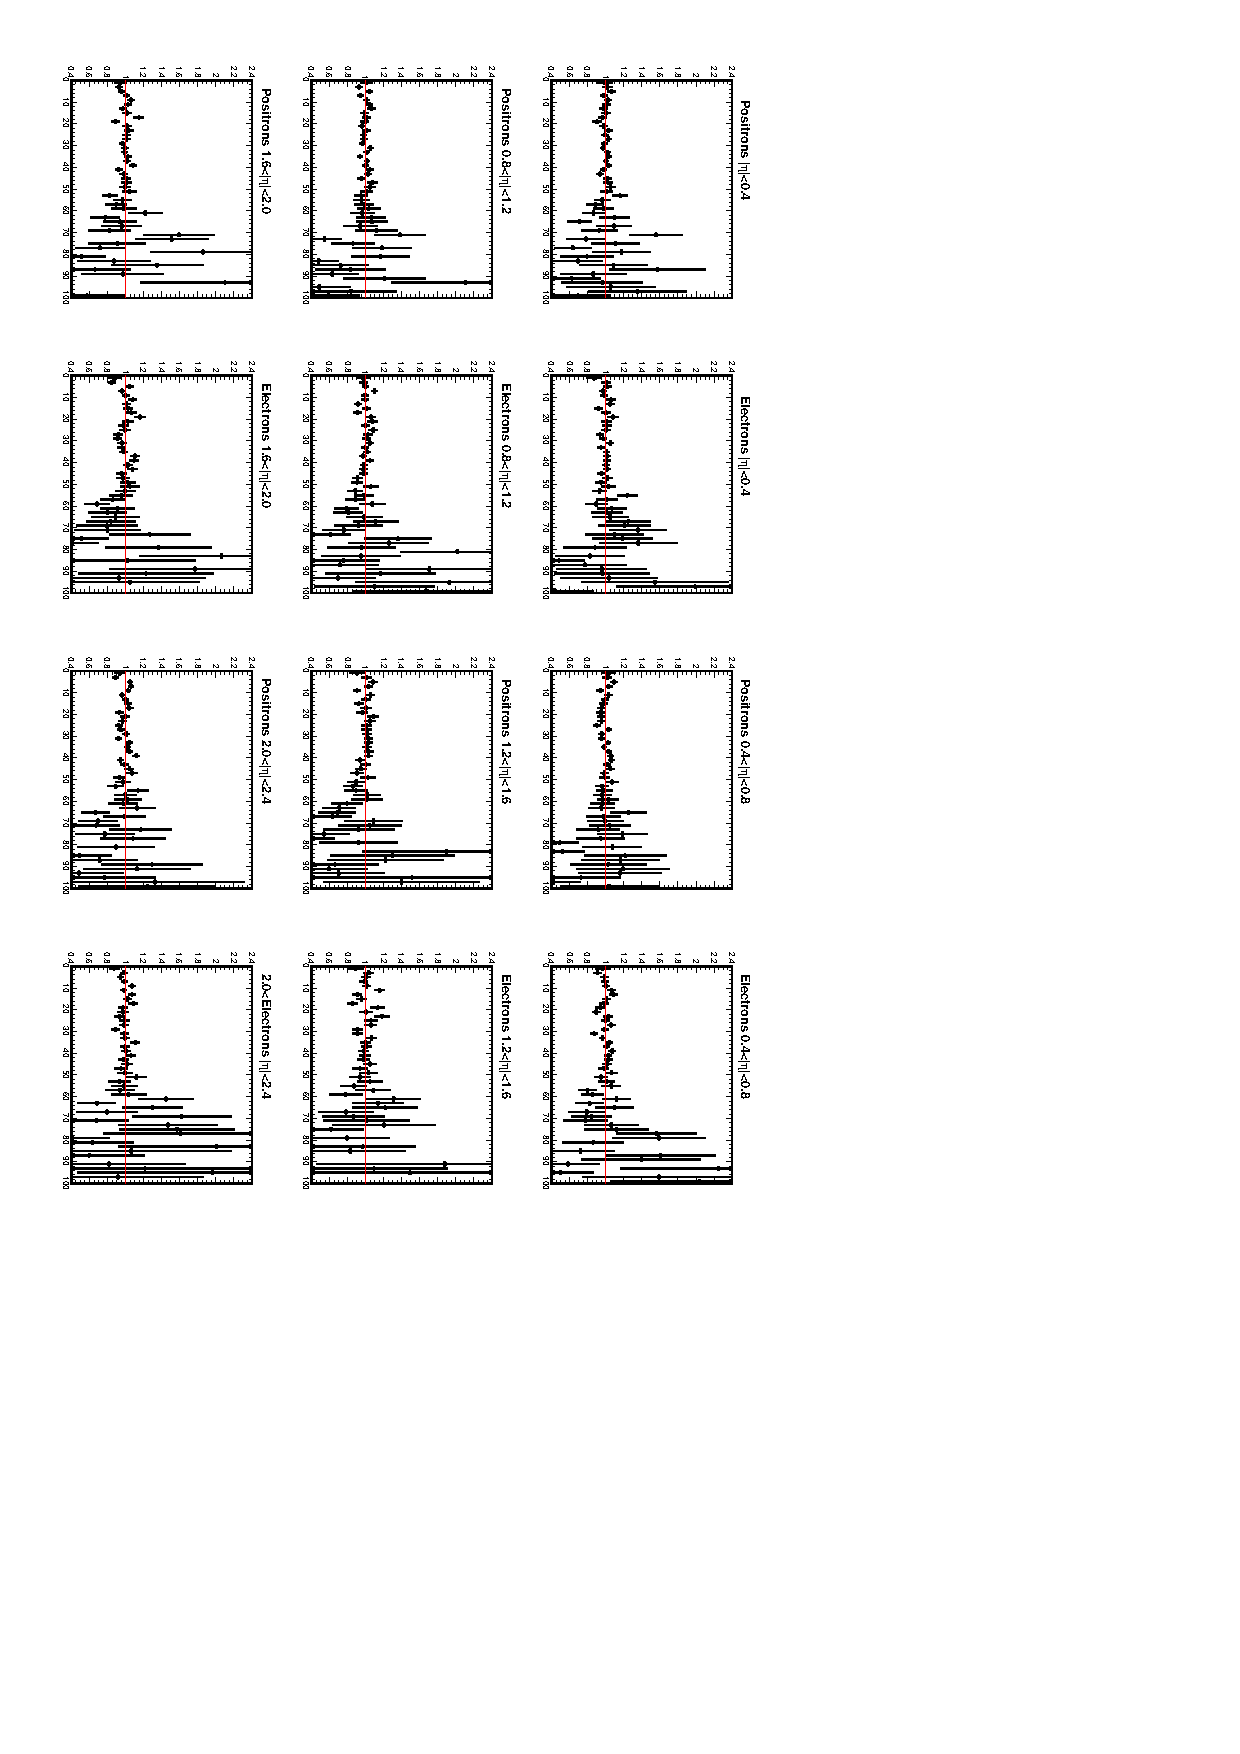
\includegraphics[trim = 0mm 0mm 80mm 100mm, clip, angle=90, width=0.95\textwidth]{Dec22_fitratio}
%\caption{\label{fig:fit2ratio}Ratio between fit and data for each
%pseudorapidity/charge bin.  The $x$-axis is the particle flow \ETm (GeV).}
%\end{center}
%\end{figure}

\clearpage

\section{\unit{840}{\invpb}}
The following plots show the results of the fits to the \ETm distribution in
each pseudorapidity/charge bin with \unit{840}{\invpb} of data. A \pT cut of
\unit{35}{\GeV} is applied. The $x$-axis is the particle flow \ETm (GeV) and the
$y$-axis is the number of events ($\GeV^{-1}$).

\begin{figure}[htb]
\begin{center}
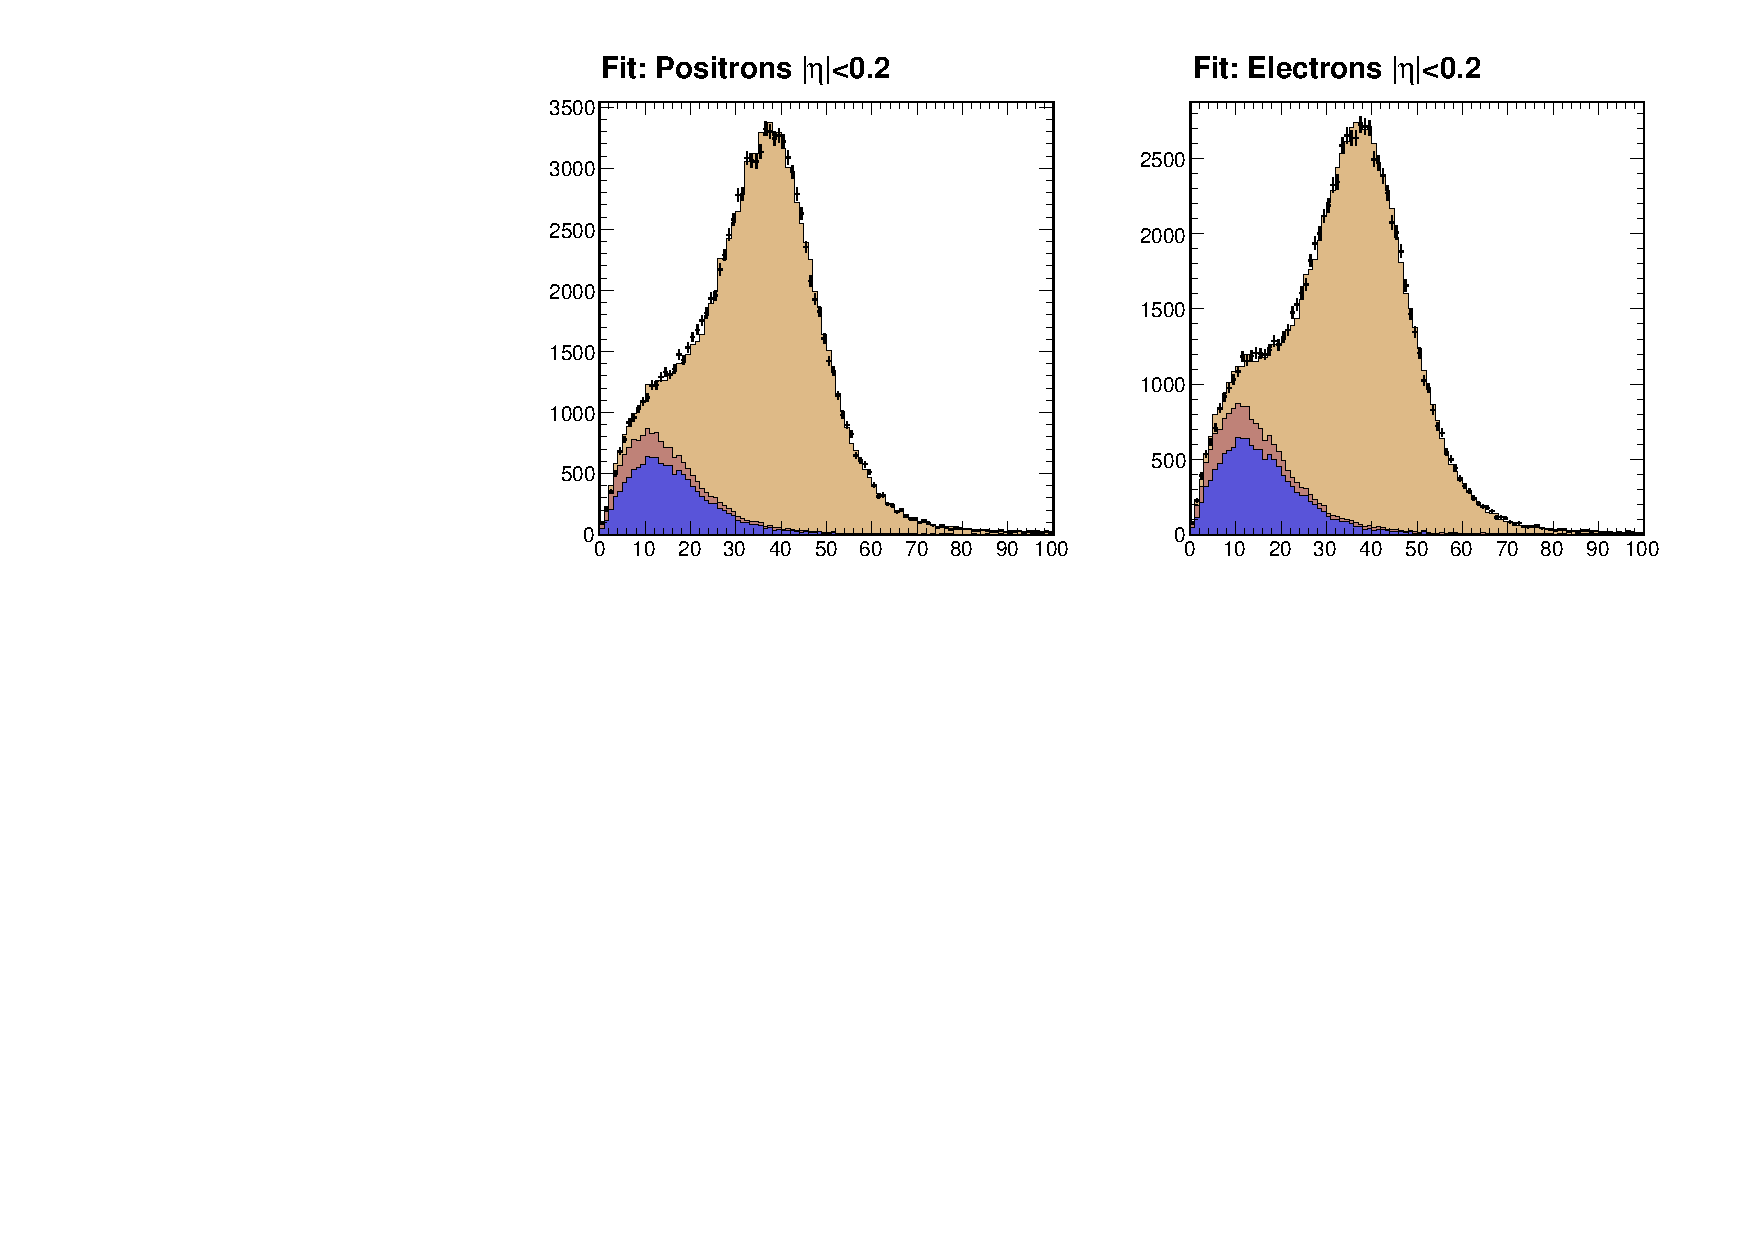
\includegraphics[width=0.95\textwidth]{data_0.pdf} \\
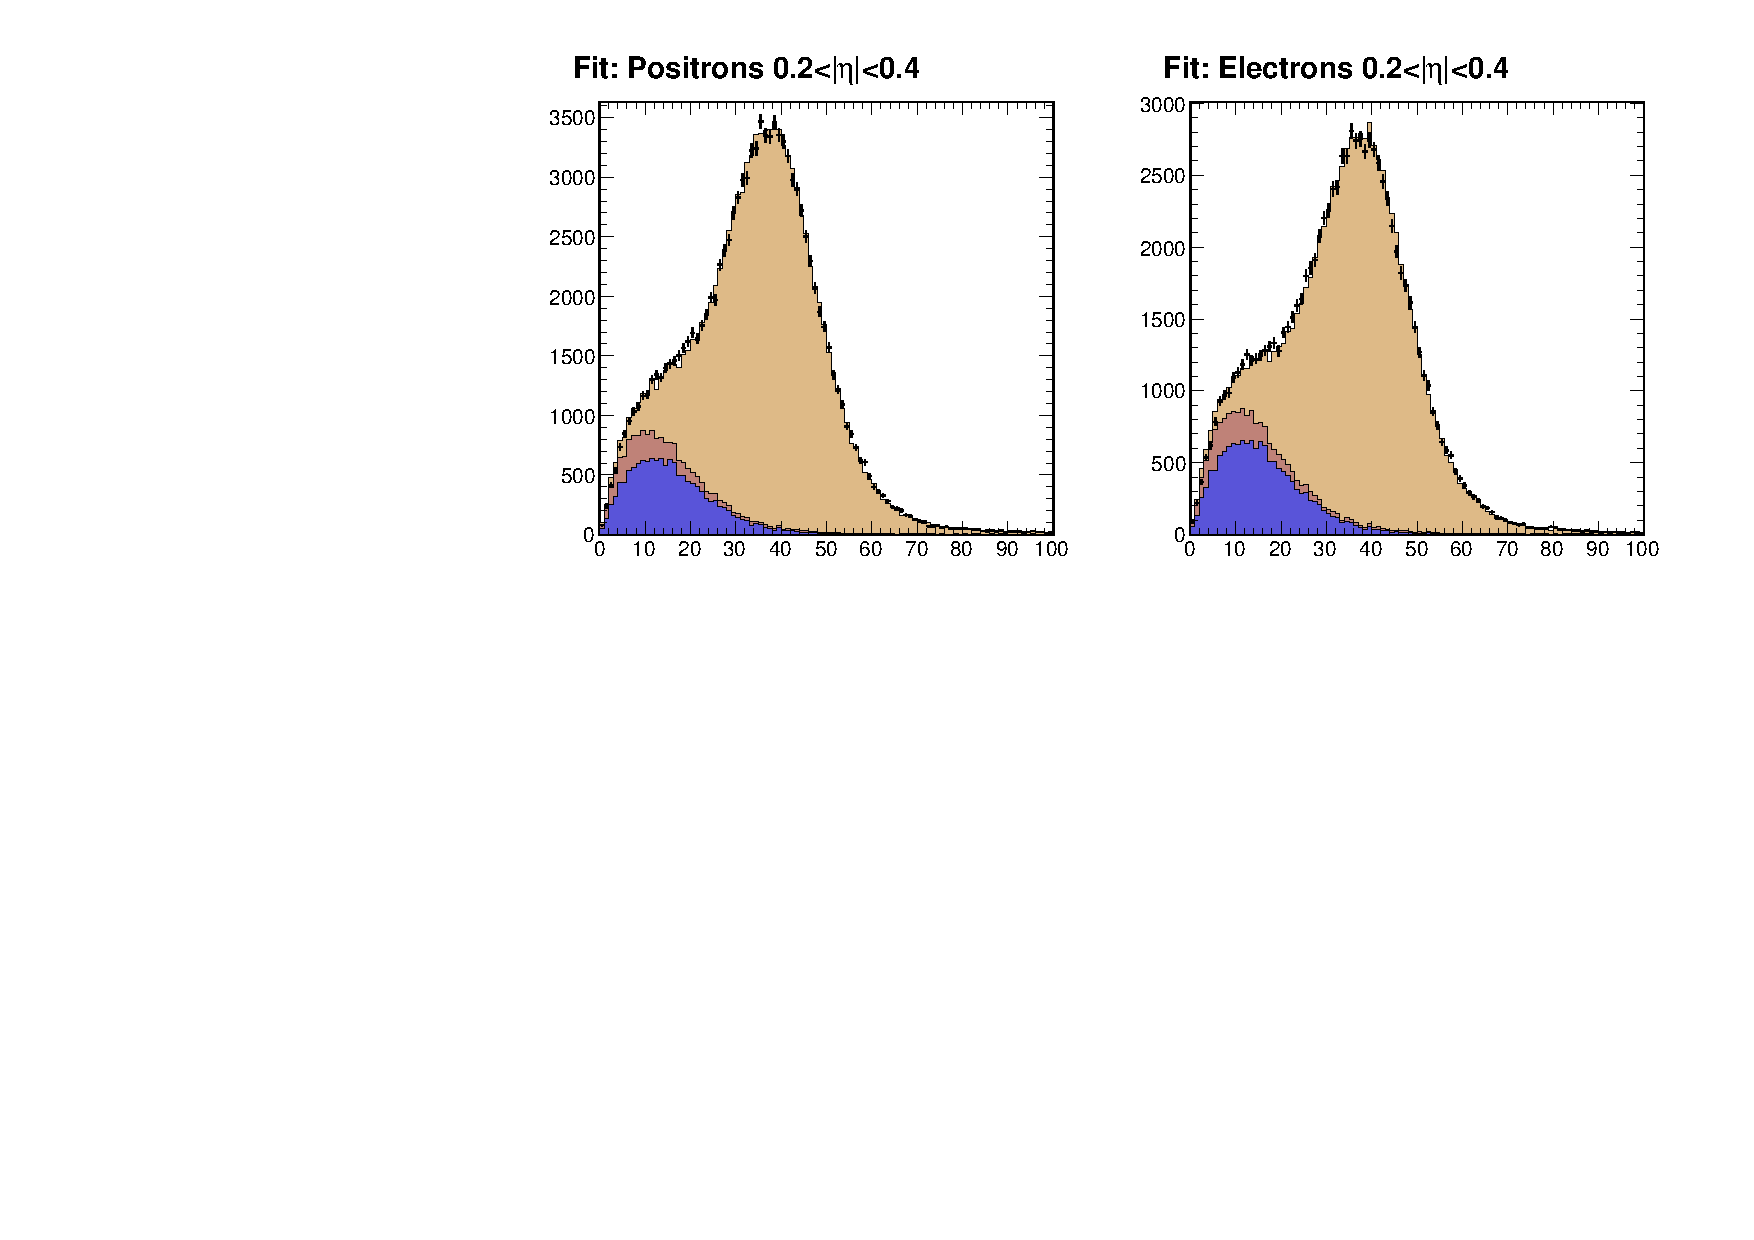
\includegraphics[width=0.95\textwidth]{data_1.pdf} \\
\caption[The fit to \MET for pseudorapidity bins 1 and 2.]
{\label{fig:data1} The fit to \MET\ for pseudorapidity bins 1,2 and
3.  The $x$-axis is the particle flow \ETm (GeV) and the $y$-axis is the number
of events ($\GeV^{-1}$).}
\end{center}
\end{figure}

\begin{figure}
\begin{center}
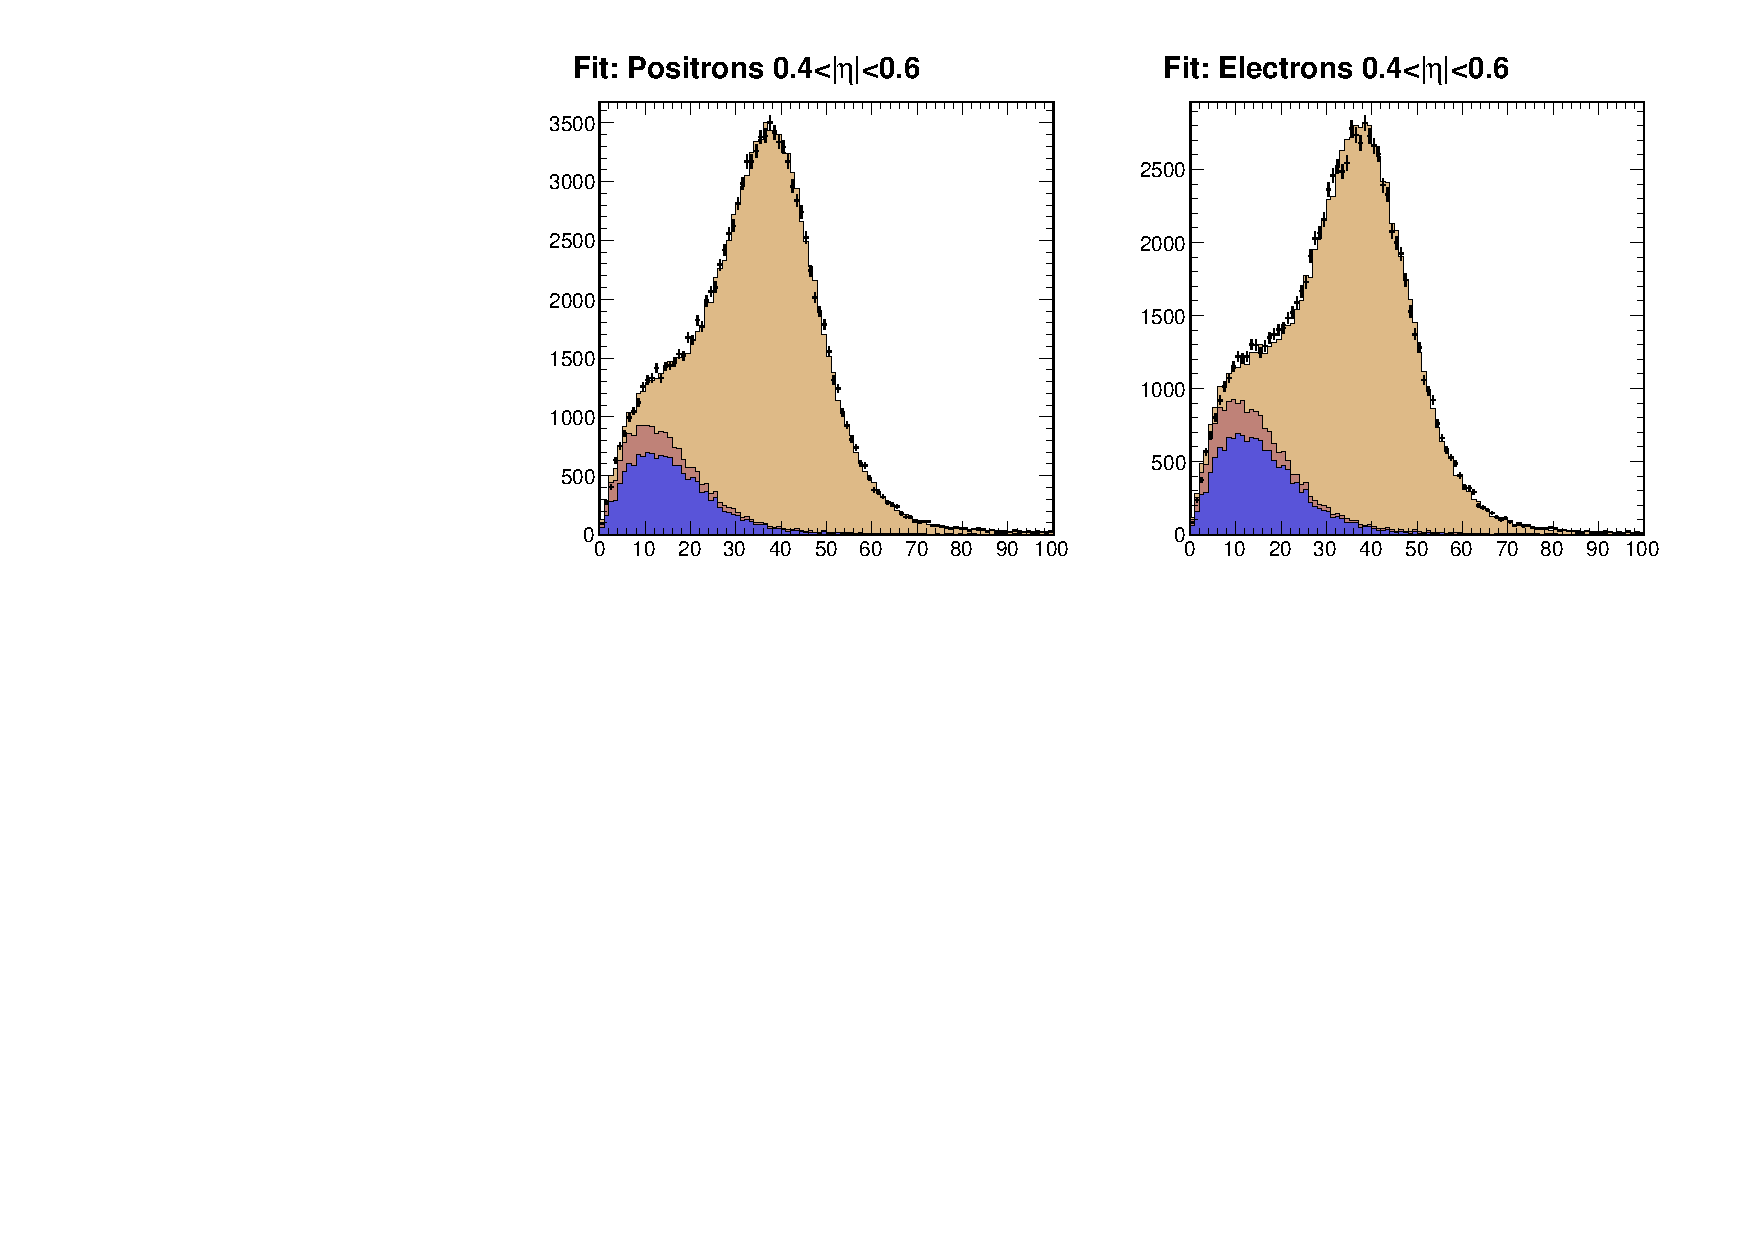
\includegraphics[width=0.95\textwidth]{data_2.pdf}
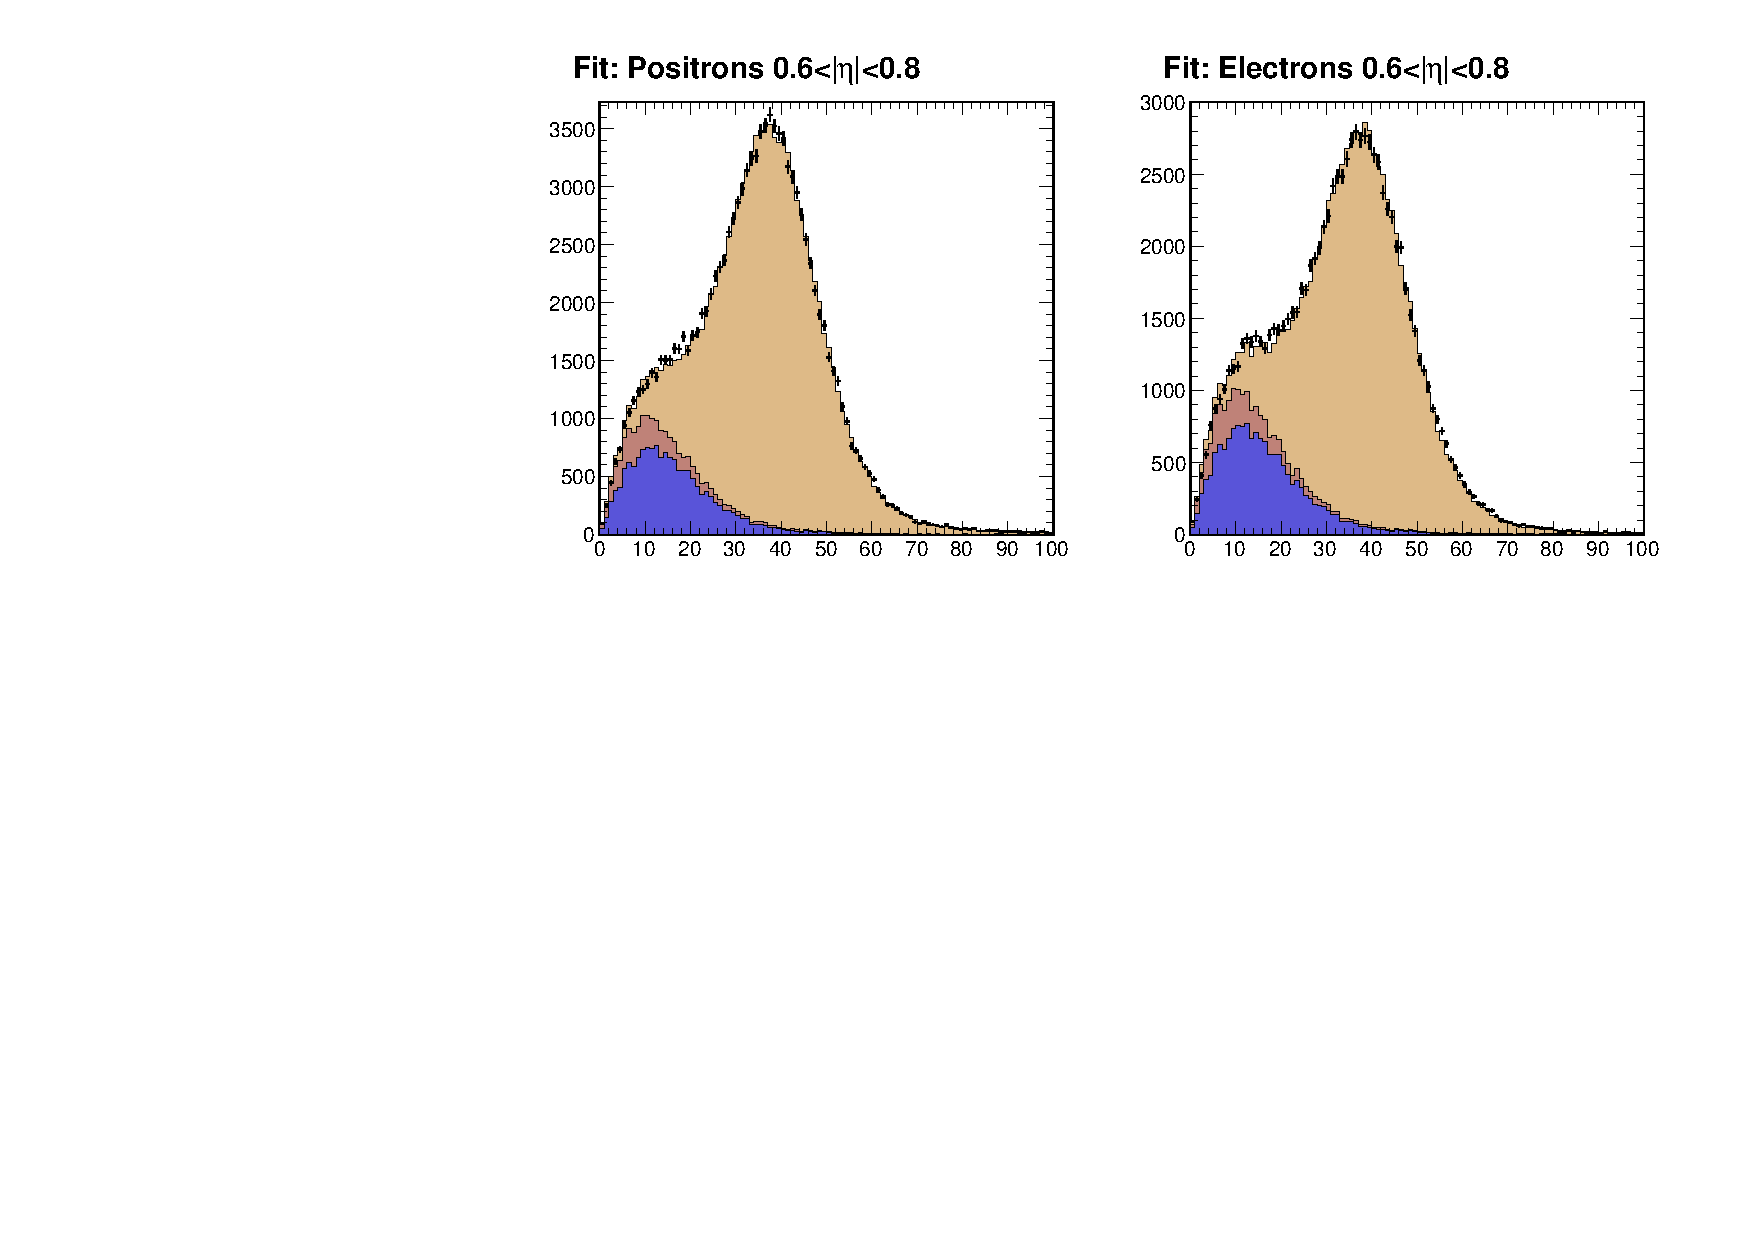
\includegraphics[width=0.95\textwidth]{data_3.pdf} \\
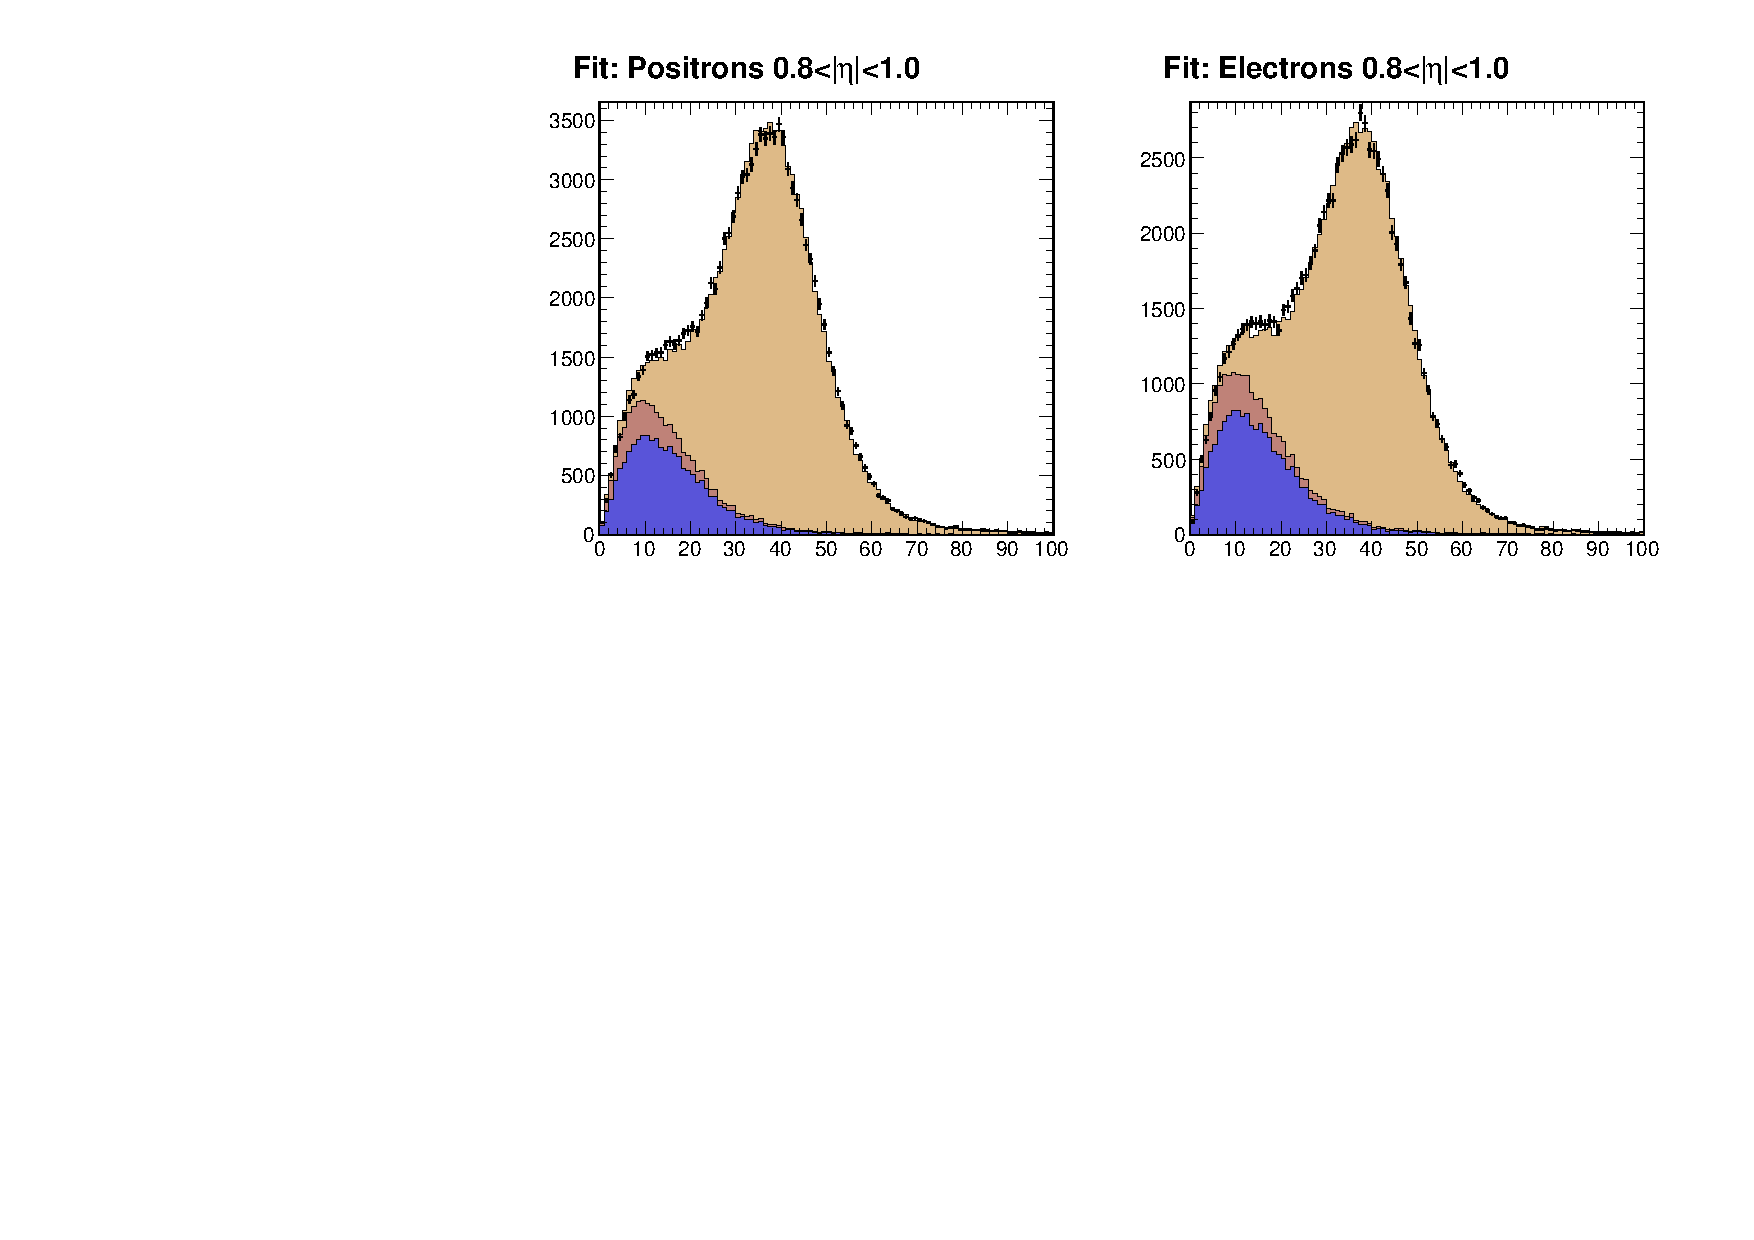
\includegraphics[width=0.95\textwidth]{data_4.pdf} \\
\caption[The fit to \MET for pseudorapidity bins 3,4 and 5.]
{\label{fig:data2} The fit to \MET\ for pseudorapidity bins 4,5 and
6.  The $x$-axis is the particle flow \ETm (GeV) and the $y$-axis is the number
of events ($\GeV^{-1}$).}
\end{center}
\end{figure}

\begin{figure}
\begin{center}
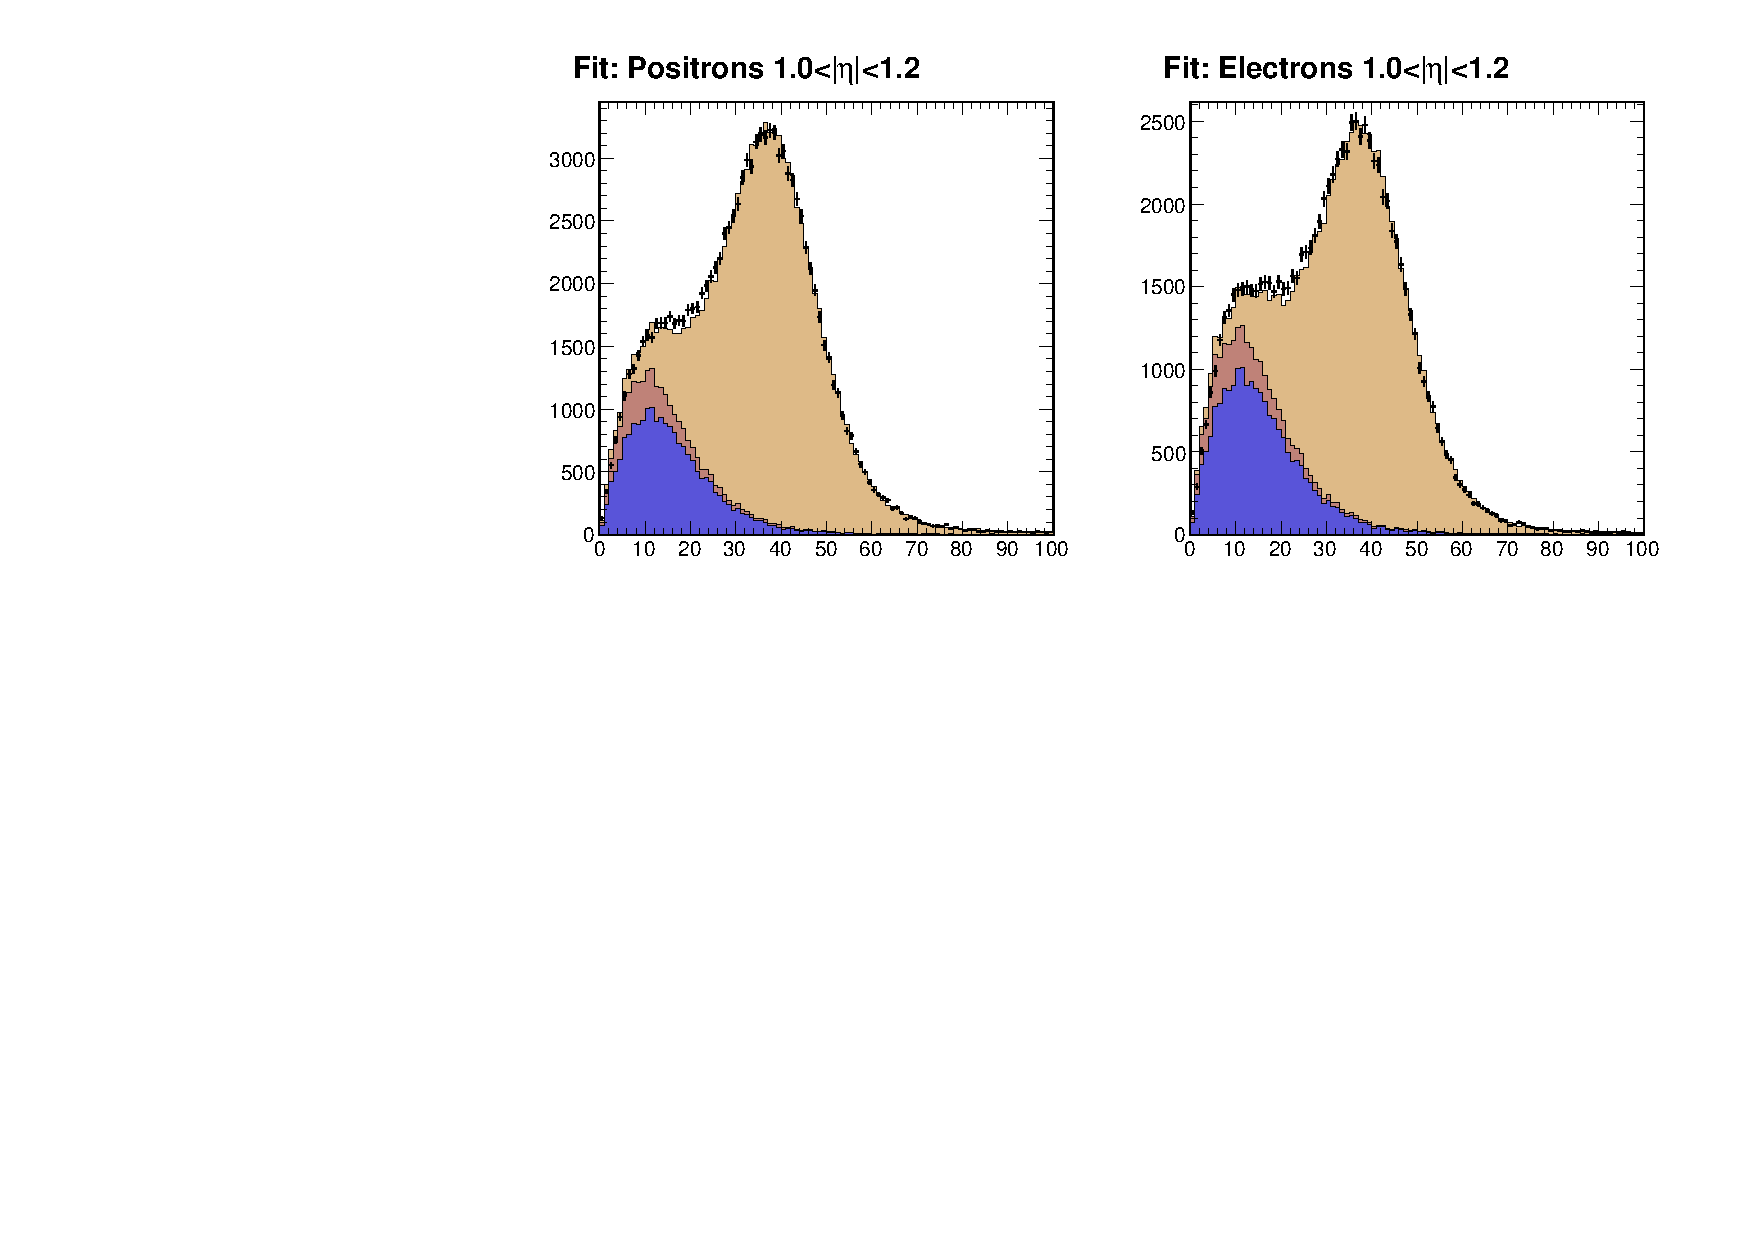
\includegraphics[width=0.95\textwidth]{data_5.pdf}
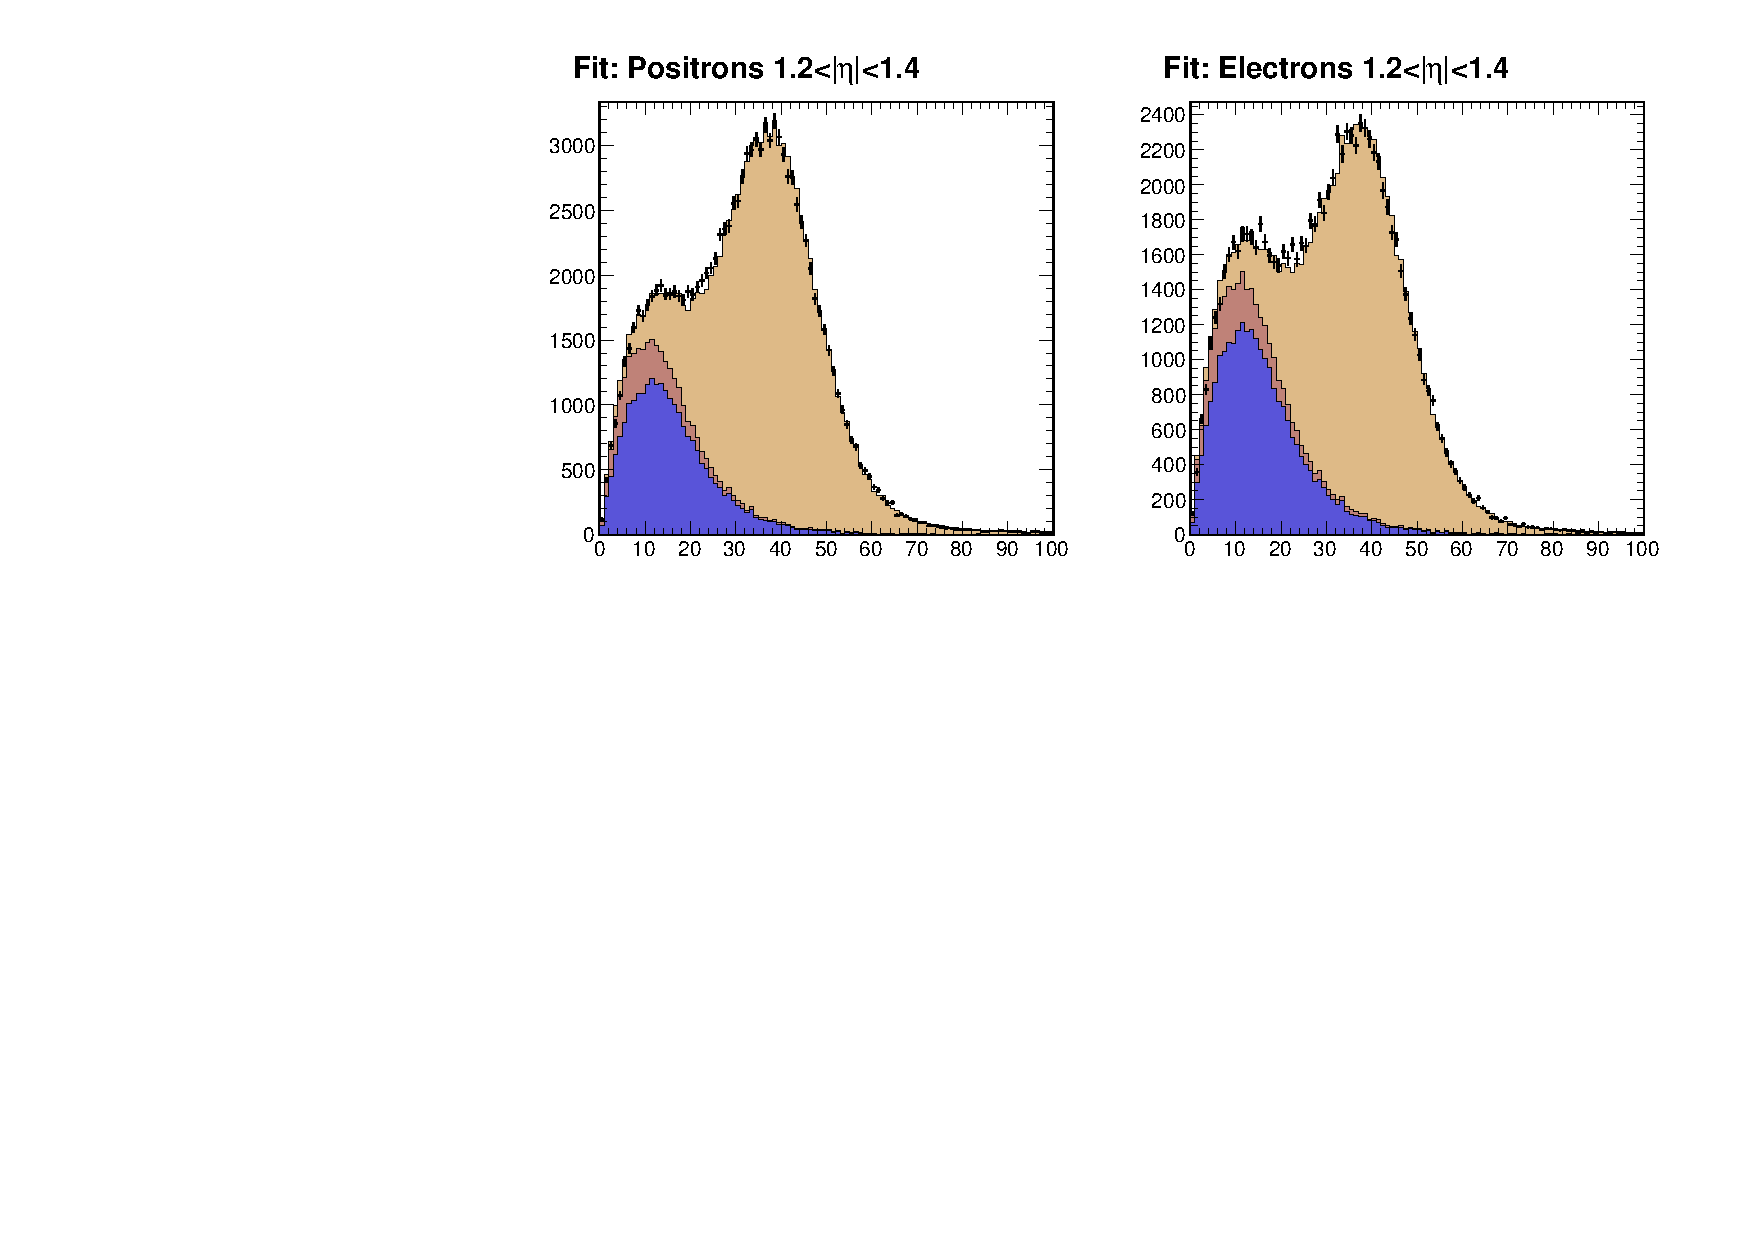
\includegraphics[width=0.95\textwidth]{data_6.pdf} \\
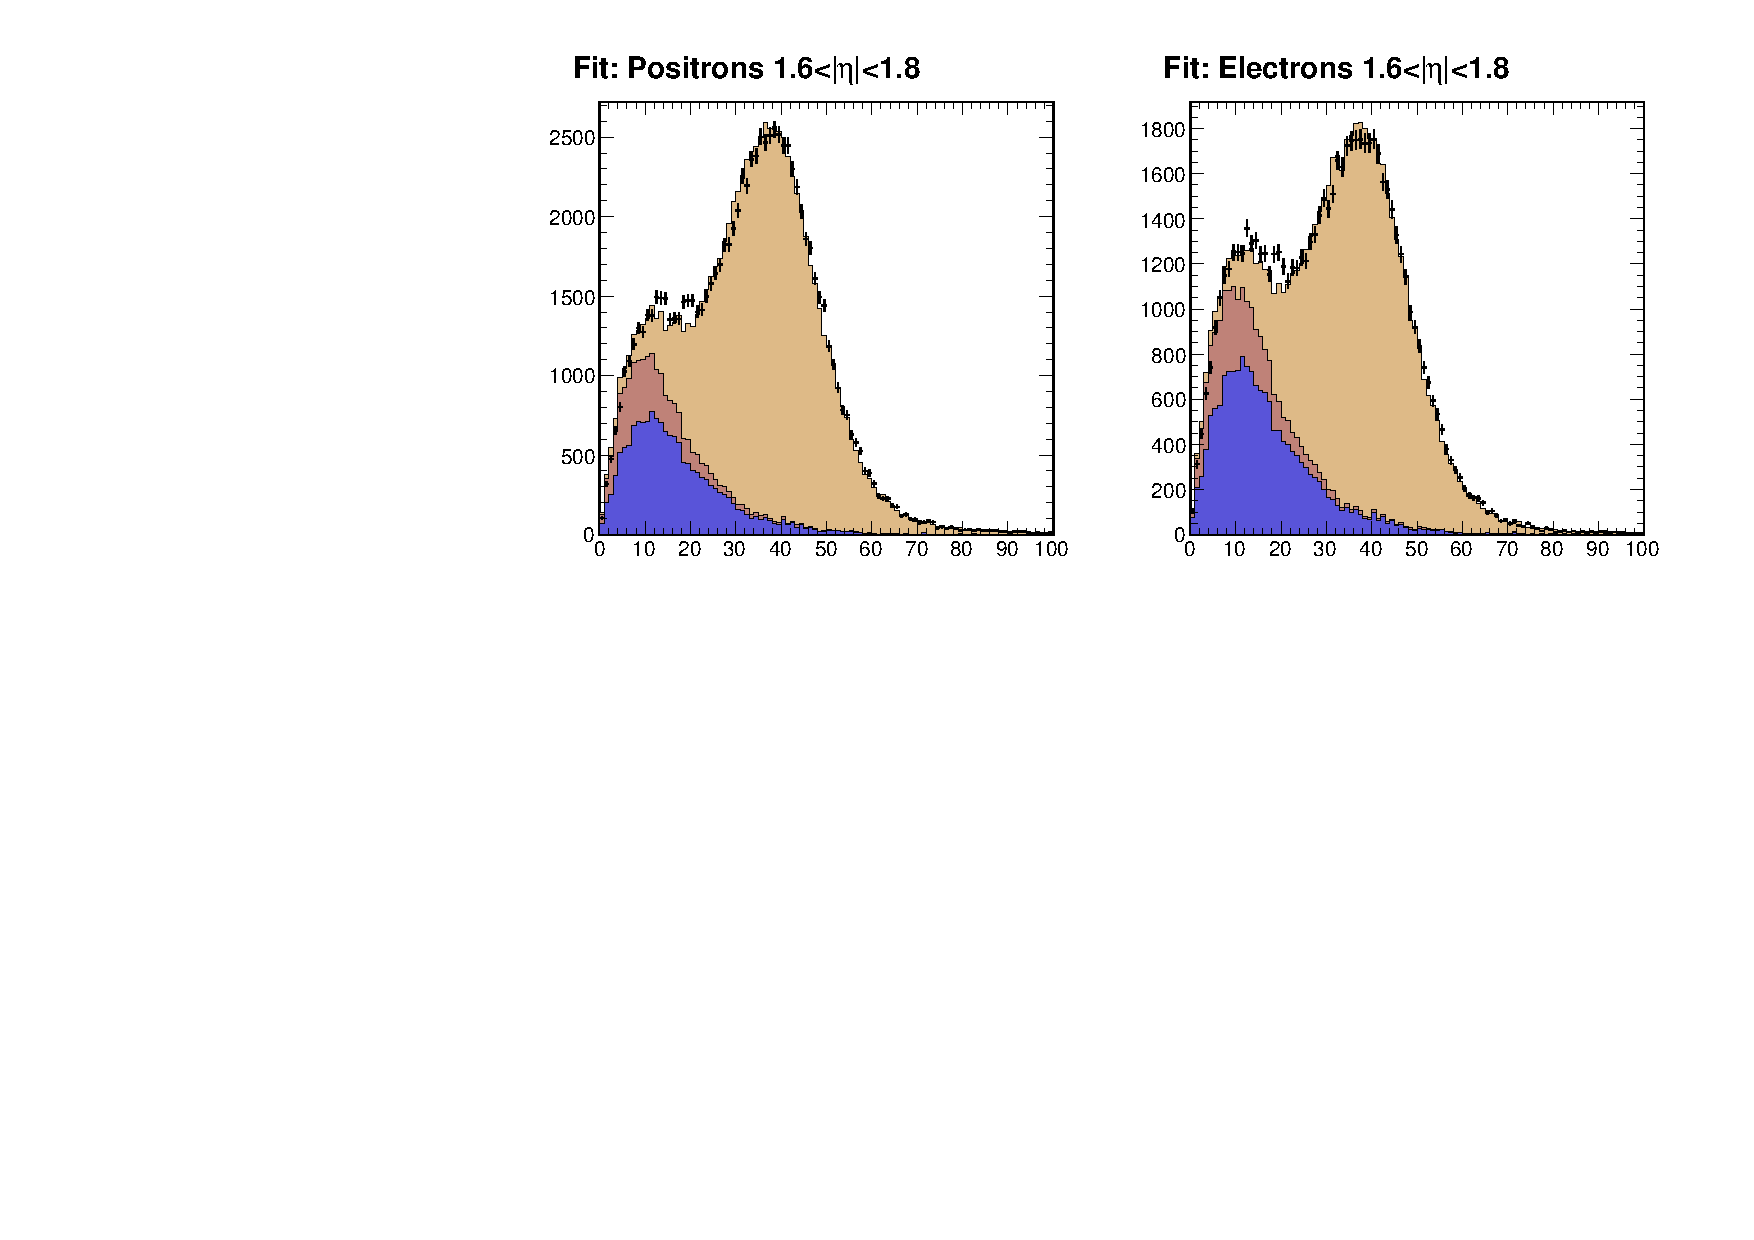
\includegraphics[width=0.95\textwidth]{data_7.pdf} \\
\caption[The fit to \MET for pseudorapidity bins 6,7 and 8.]
{\label{fig:data3} The fit to \MET\ for pseudorapidity bins 7,8 and
9.  The $x$-axis is the particle flow \ETm (GeV) and the $y$-axis is the number
of events ($\GeV^{-1}$).}
\end{center}
\end{figure}

\begin{figure}
\begin{center}
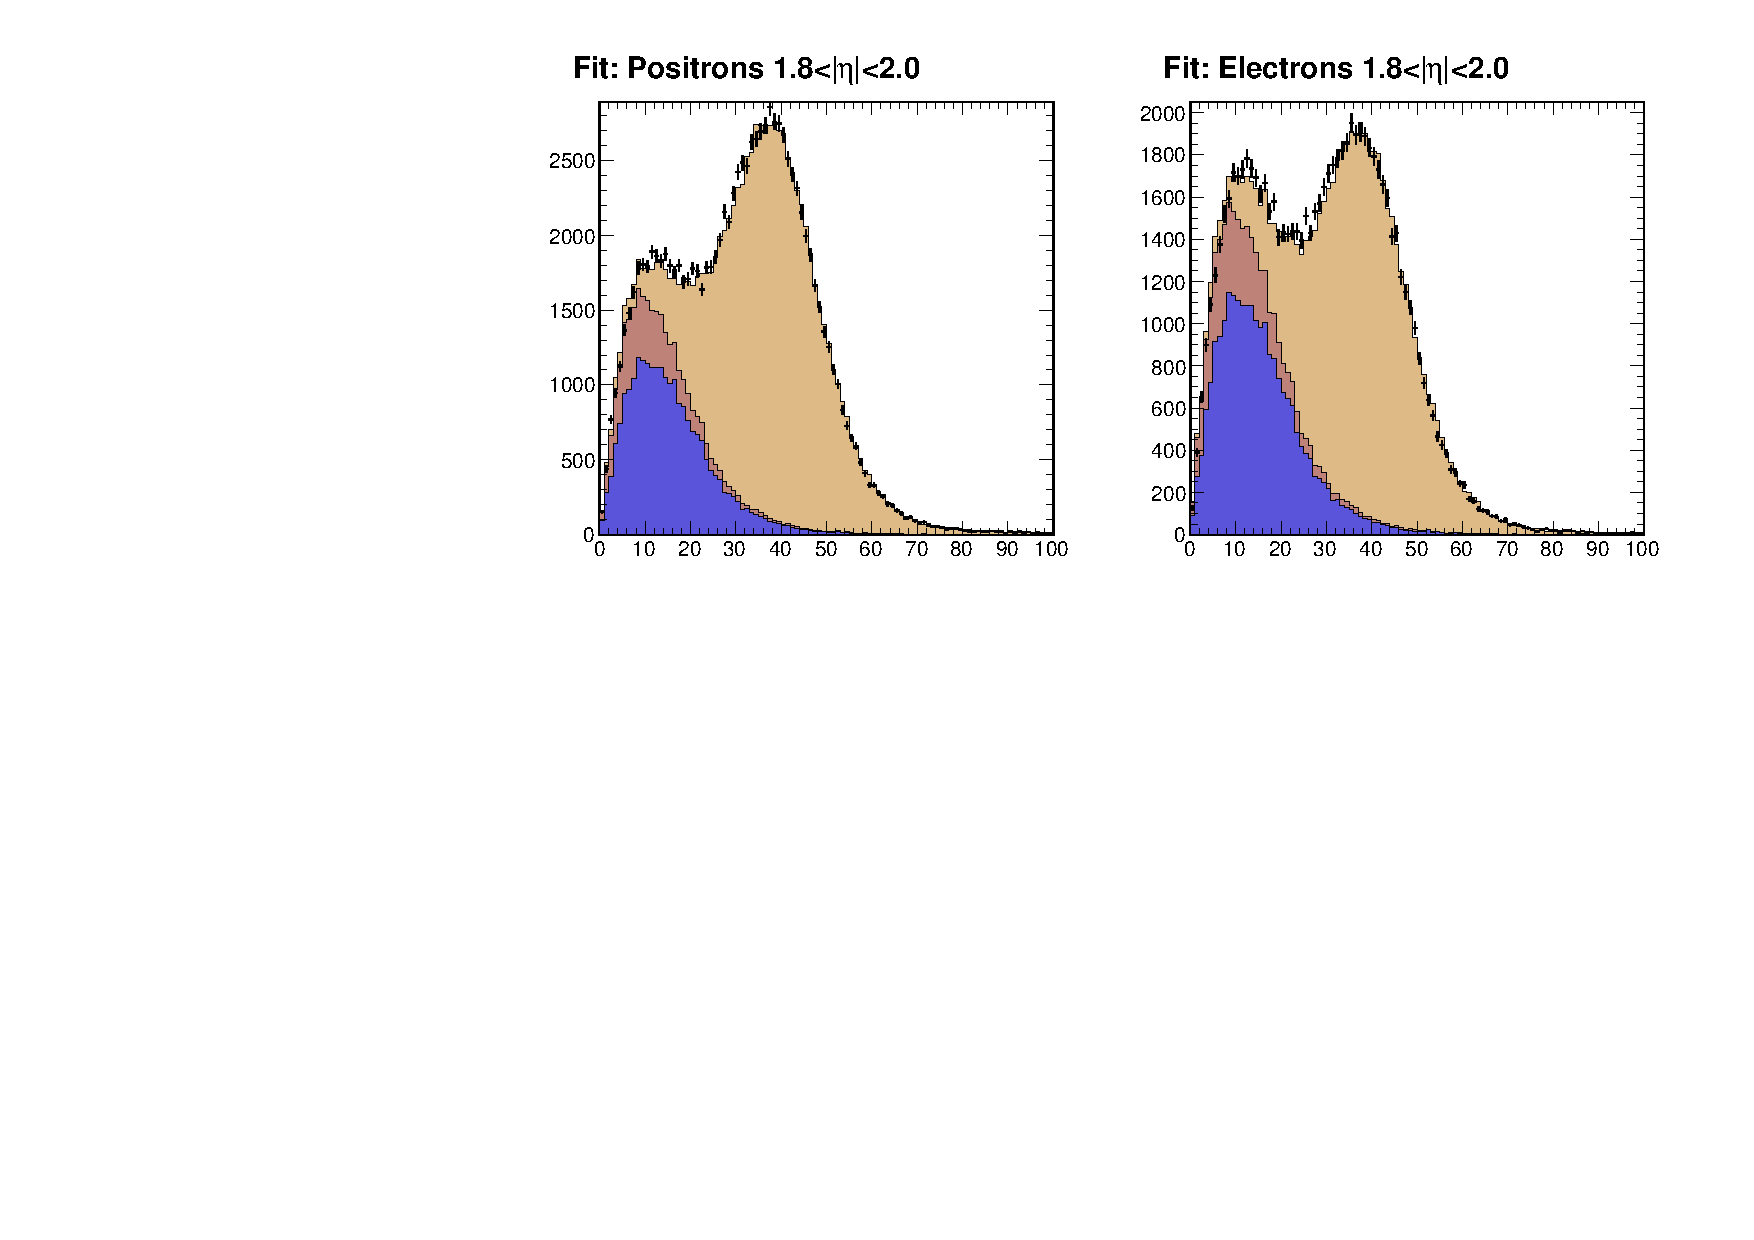
\includegraphics[width=0.95\textwidth]{data_8.pdf}
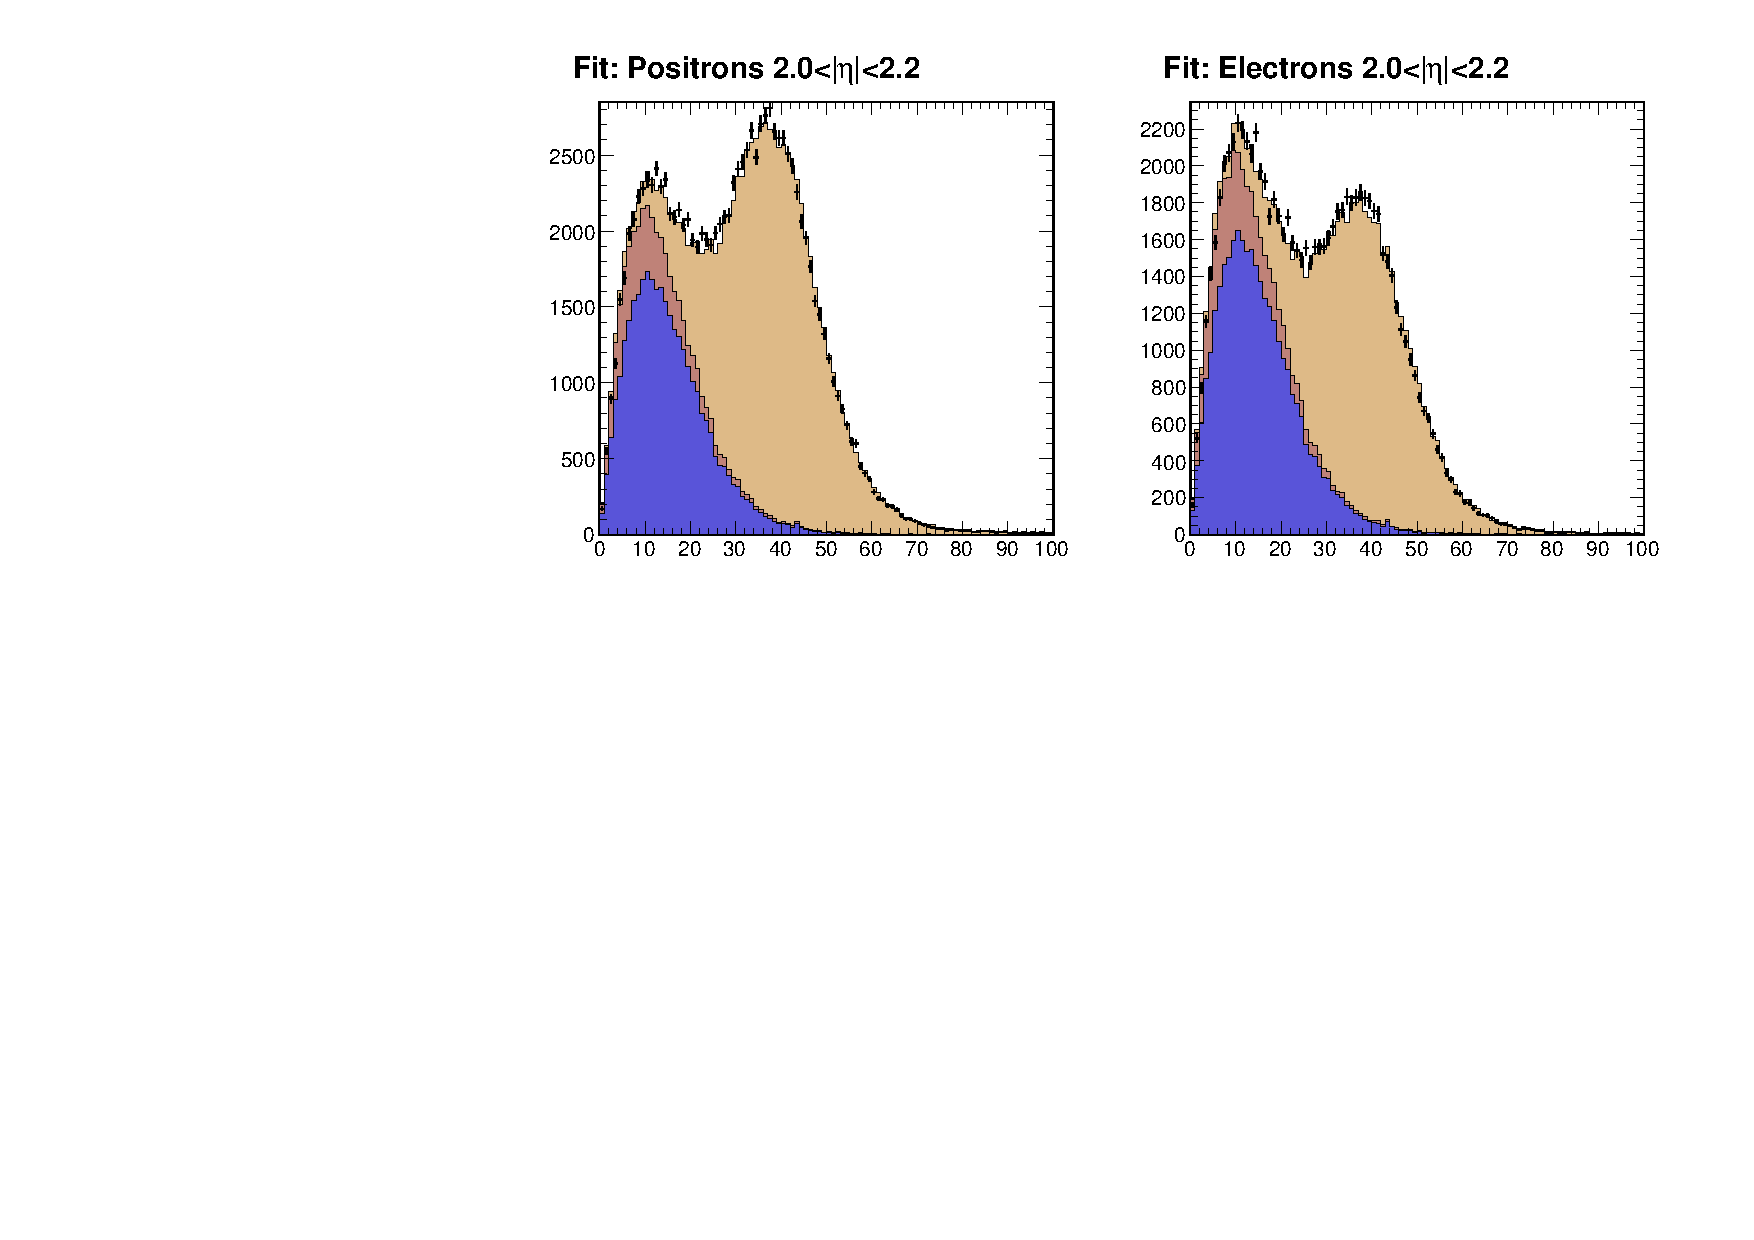
\includegraphics[width=0.95\textwidth]{data_9.pdf} \\
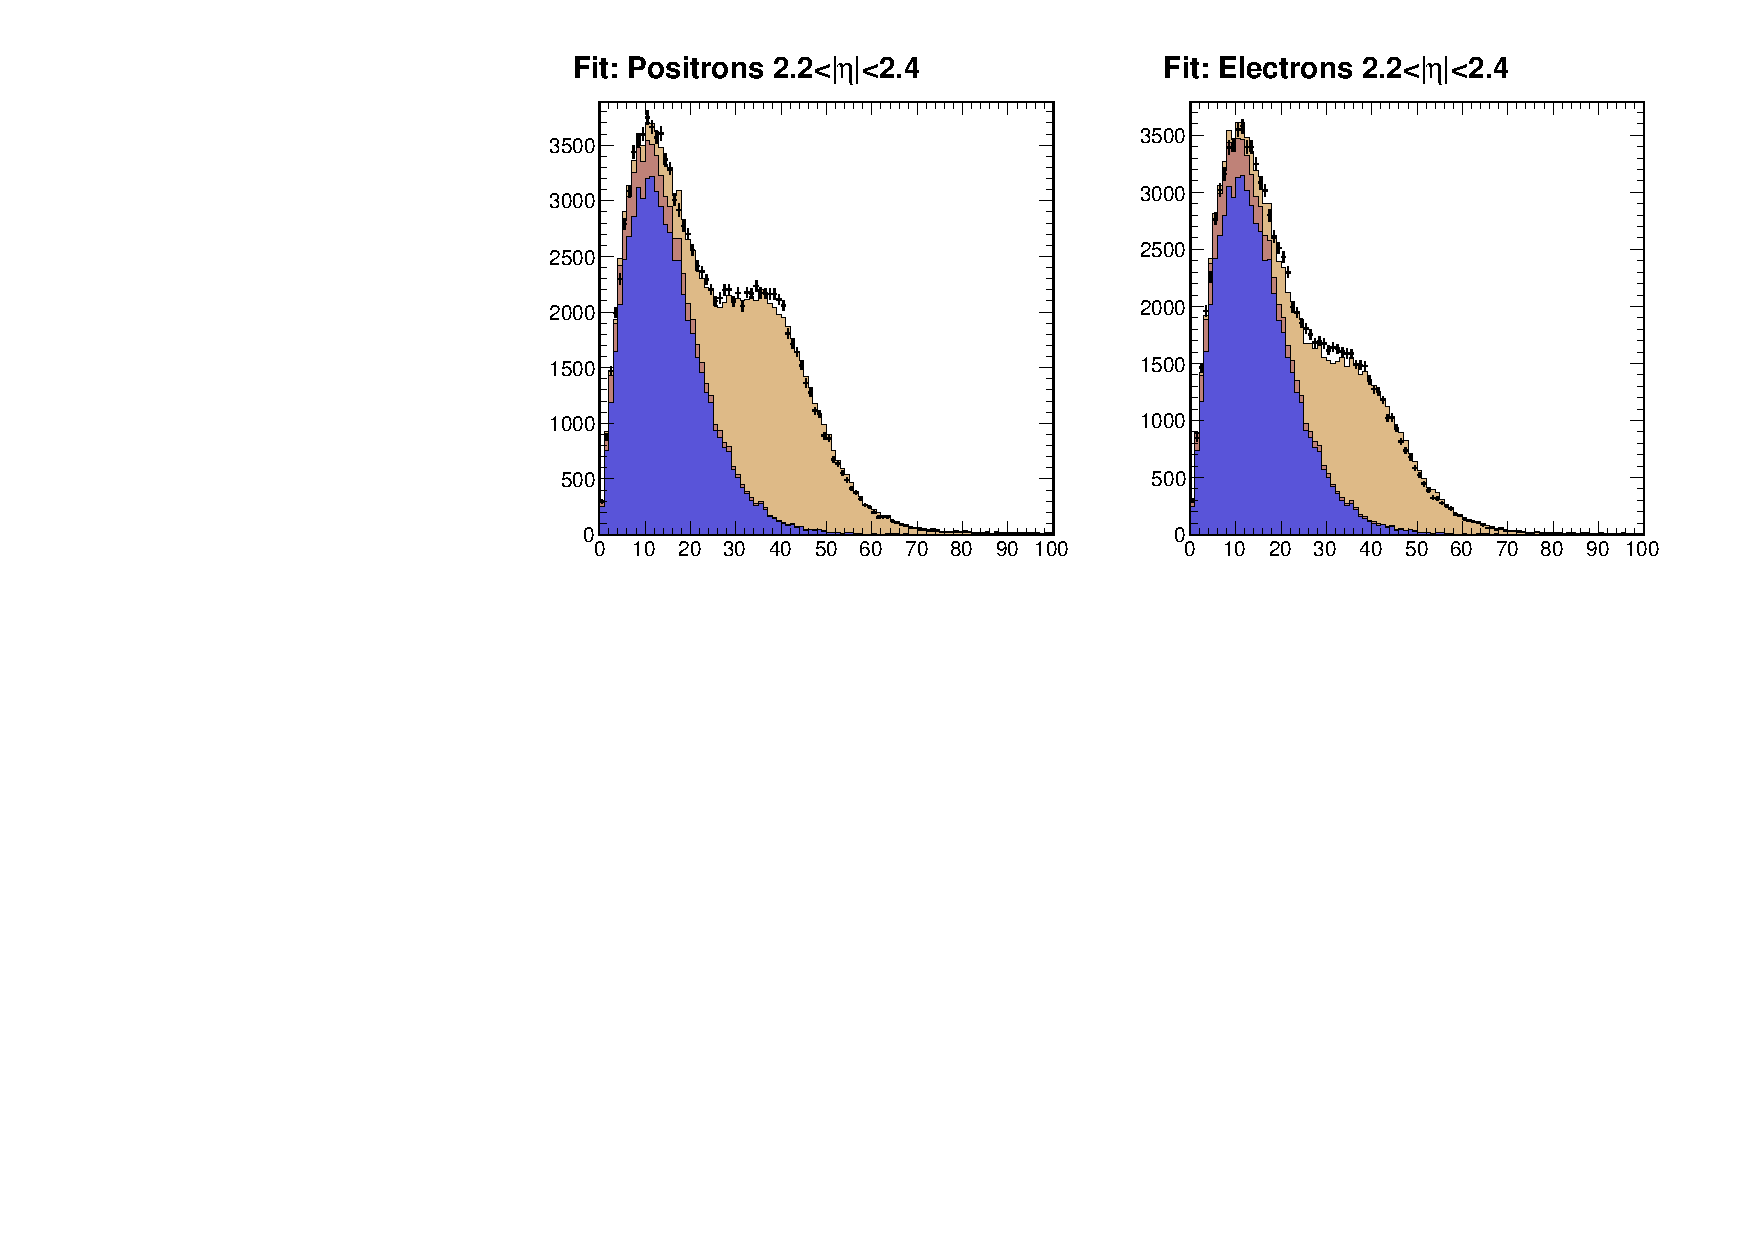
\includegraphics[width=0.95\textwidth]{data_10.pdf}
\caption[The fit to \MET for pseudorapidity bins 9,10 and 11.]
{\label{fig:data4} The fit to \MET\ for pseudorapidity bins 10 and
11.  The $x$-axis is the particle flow \ETm (GeV) and the $y$-axis is the number
of events ($\GeV^{-1}$).}
\end{center}
\end{figure}

\chapter{Monte Carlo Samples }
Monte Carlo (MC) simulation samples have been used to develop analysis
techniques and estimate some of the background contributions. 
The samples used in this thesis are sumarised in Tables \ref{tab:samples36} and
\ref{tab:samples840}.  Several different MC simulations have been used to cross-check MC
predictions and help assigning experimental systematic uncertainties.

The next-to-leading order (NLO) MC simulations based on the
{POWHEG}\cite{powheg}, {PYTHIA}\cite{pythia} or {MadGraph}\cite{madgraph} event
generators.  
The QCD multijet backgrounds are generated with the {PYTHIA} event generator.
Taus are simulated using {TAUOLA}\cite{tauola}.  
All generated events are passed through the CMS detector simulation using
{Geant4} \cite{geant} and then processed using a reconstruction sequence
identical to that used for collision data. 

\newpage
\section{\unit{36}{\invpb}}

\begin{table}[htbp]
\begin{center}
%\begin{sideways}
\small{
\begin{tabular}{ll}
\toprule
Sample & Dataset \\
\midrule
$W^+ \rightarrow e^+\nu$ 
  & {WPlusToENu\_CT10\_TuneZ2\_7TeV-powheg-pythia}\\
$W^- \rightarrow e^-\nu$ 
  & {WPlusToENu\_CT10\_TuneZ2\_7TeV-powheg-pythia}\\
$W \rightarrow \tau \nu$ 
  & {WToTauNu\_TuneZ2\_7TeV-pythia6-tauola}\\
DY $M_{e^+e^-}>20$ \GeV 
  & {DYToEE\_M-20\_CT10\_TuneZ2\_7TeV-powheg-pythia}\\
DY $M_{\tau^+\tau^-}>20$\GeV
  & {DYToTauTau\_M-20\_CT10\_TuneZ2\_7TeV-tauola}\\
$t\bar{t}$ + jets 
  & {TT\_TuneZ2\_7TeV-pythia6-tauola}\\
QCD EM-enr $20<\hat{pt}<30$ \GeV 
  & {QCD\_Pt-20to30\_EMEnriched\_TuneZ2\_7TeV-pythia6}\\
QCD EM-enr $30<\hat{pt}<80$ \GeV 
  & {QCD\_Pt-30to80\_EMEnriched\_TuneZ2\_7TeV-pythia6}\\
QCD EM-enr $80<\hat{pt}<170$ \GeV
  & {QCD\_Pt-80to170\_EMEnriched\_TuneZ2\_7TeV-pythia6}\\
QCD ($b,c\rightarrow e$) $20<\hat{pt}<30$ \GeV
  & {QCD\_Pt-20to30\_BCtoE\_TuneZ2\_7TeV-pythia6}\\
QCD ($b,c\rightarrow e$) $30<\hat{pt}<80$ \GeV  
  & {QCD\_Pt-30to80\_BCtoE\_TuneZ2\_7TeV-pythia6}\\
QCD ($b,c\rightarrow e$) $80<\hat{pt}<170$ \GeV
  & {QCD\_Pt-80to170\_BCtoE\_TuneZ2\_7TeV-pythia6}\\
$\gamma$ + jets $30 <\hat{pt} <50$ \GeV  
  & {G\_Pt\_30to50\_TuneZ2\_7TeV\_pythia6}\\
$\gamma$ + jets $50 <\hat{pt} < 80$ \GeV 
  & {G\_Pt\_50to80\_TuneZ2\_7TeV\_pythia6} \\
\bottomrule
\end{tabular}
}
%\end{sideways}
\caption[The Monte Carlo (MC) samples used in the \unit{36}{\invpb}
measurement.] {\label{tab:samples36} The Monte Carlo (MC) samples used in the
\unit{36}{\invpb} measurement. 
The QCD EM-enr are samples of QCD that have been
enriched with EM events.  The Drell-Yan (DY) samples include
\HepProcess{\PZ\to\Plepton\Plepton} and
\HepProcess{\Pphoton\to\Plepton\Plepton}.
 All the samples are from the
\emph{Fall10} MC production.}
\end{center} 
\end{table}

\newpage
\section{\unit{840}{\invpb}}

\begin{table}[htbp]
\begin{center}
%\begin{sideways}
\small{
\begin{tabular}{ll}
\toprule
Sample & Dataset\\ % & $N_{events}$ & $\sigma$ (pb) \\
\midrule
\multicolumn{2}{l}{\emph{PYTHIA}} \\ 
$W \rightarrow e \nu$
   & WToENu\_TuneZ2\_7TeV\_pythia6\\
$W \rightarrow \tau \nu$ 
   & WToTauNu\_TuneZ2\_7TeV\_pythia6\_tauola\\
$t\bar{t}$ + jets       
   & TT\_TuneZ2\_7TeV\_pythia6\_tauola\\
{QCD EM-enr}  $20<\hat{pt}<30$ GeV       
   & QCD\_Pt-20to30\_EMEnriched\_TuneZ2\_7TeV\_pythia6\\
{QCD EM-enr}  $30<\hat{pt}<80$  GeV     
   & QCD\_Pt-30to80\_EMEnriched\_TuneZ2\_7TeV\_pythia6\\
{QCD EM-enr}  $80<\hat{pt}<170$   GeV   
   & QCD\_Pt-80to170\_EMEnriched\_TuneZ2\_7TeV\_pythia6\\
{QCD ($b,c\rightarrow e$)}  $20<\hat{pt}<30$ GeV 
   & QCD\_Pt-20to30\_BCtoE\_TuneZ2\_7TeV-pythia6\\
{QCD ($b,c\rightarrow e$)}  $30<\hat{pt}<80$ GeV 
   & QCD\_Pt-30to80\_BCtoE\_TuneZ2\_7TeV-pythia6\\
{QCD ($b,c\rightarrow e$)}  $80<\hat{pt}<170$ GeV 
   & QCD\_Pt-80to170\_BCtoE\_TuneZ2\_7TeV-pythia6\\
{$\gamma$ + jets  } $50 <\hat{pt} < 80$ GeV       
   & G\_Pt-50to80\_TuneZ2\_7TeV\_pythia6\\
\multicolumn{2}{l}{\emph{MadGraph}} \\ 
$W \rightarrow \ell \nu$ 
   & WJetsToLNu\_TuneZ2\_7TeV\_madgraph\_tauola\\
DY $\rightarrow \ell^+\ell^-$	 
   & DYJetsToLL\_TuneZ2\_M\_50\_7TeV\_madgraph\_tauola\\
$t\bar{t}$ + jets        
   & TTJets\_TuneZ2\_7TeV\_madgraph\_tauola\\
\bottomrule
\end{tabular}
}
%\end{sideways}
\caption[Monte Carlo samples used in the \unit{840}{\invpb} measurement. ]
{\label{tab:samples840}Monte Carlo samples used in the \unit{840}{\invpb}
measurement. All samples are from the \emph{Summer11} MC production. 
} 

\end{center}
\end{table}
